\chapter{BugMentor: Answering Follow-up Questions from Bug Reports Leveraging Structured Information Retrieval with Neural Text Generation}\label{chapter:BugMentor}


% \begin{abstract}
\looseness=-1
Software bug reports often lack crucial information (e.g., steps to reproduce), which makes bug resolution challenging. Developers thus ask follow-up questions to capture additional information. However, according to existing evidence, bug reporters often face difficulties answering them, which leads to the premature closing of bug reports without any resolution. Recent studies suggest follow-up questions to support the developers, but answering the follow-up questions still remains a major challenge. In this chapter, we propose BugMentor, a novel approach that combines neural text generation (e.g., CodeT5) and structured information retrieval to generate appropriate answers to the follow-up questions. 

The rest of this chapter is organized as follows. Section~\ref{Chap1:Intro} introduces our study and discusses the novelty of our work. Section~\ref{sec:motivating-example} discusses a motivating example to demonstrate the effectiveness of BugMentor. Section~\ref{Chap1:BugMentor} discusses our proposed technique. Section~\ref{Chap1:Experiment} presents our experimental design, datasets, and evaluation metrics. Section~\ref{Chap1:Evaluation} discusses the evaluation results of BugMentor. Section~\ref{Chap1:RelatedWork} discusses relevant works to our study. Section~\ref{Chap1:Threats} discusses the threats to the validity of our study. Finally, Section~\ref{Chap1:Summary} summarizes this study.

\section{Introduction} \label{Chap1:Intro}

\looseness=-1
Software bugs are human-made errors in a software system that prevent the software from working as expected~\cite{ieeestandardglossaryforse}. Studies have shown that software bugs cost the global economy billions of dollars every year~\cite{britton2013reversible, zou2018practitioners}. Developers also spend $\sim$50\% of their programming time finding and fixing bugs~\cite{britton2013reversible}. Thus, bug resolution has been one of the major challenges in software maintenance~\cite{zou2018practitioners}. Hundreds of software bugs are submitted to bug-tracking systems like GitHub and JIRA as \textit{bug reports} ~\cite{anvik2006should}. These bugs are then triaged, analyzed, and resolved by developers.\par



\looseness=-1
Ideally, bug reports should contain all the information, such as system configuration, expected behaviour, observed behaviour, and reproducing steps that help a developer resolve a bug~\cite{chaparro2017detecting}. However, in practice, they often do not contain all the required information for reproducing or resolving the bug~\cite{chaparro2017detecting}. According to existing literature~\cite{chaparro2017detecting},  64.8\% of bug reports do not contain any expected behaviour of target software systems, and 48.6\% of them do not explicitly describe the steps to reproduce a bug. Missing information like this has been found to be a key factor behind the non-reproducibility of software bugs~\cite{rahman2020some}. In a survey conducted by Zou et al.~\cite{zou2018practitioners}, 77\% of 327 professional developers from the major technology companies (e.g., Google, Meta, Amazon, Microsoft) consider missing information as a major problem and emphasize on complementing bug reports with useful information (e.g., steps to reproduce, environmental configuration)~\cite{zou2018practitioners}. In short, missing information has been a key challenge toward cost-effective bug resolution. \par



\looseness=-1
Many software projects on GitHub now require bug reports to adhere to specific templates or standard guidelines~\cite{githubguidelines}. Unfortunately, many bug reporters might fail to comply with them and might not be able to provide all the information during report submission~\cite {imran2021automatically}. Developers thus often pose \textit{follow-up} questions to bug reporters soliciting the missing information. Unfortunately, the bug reporters often find it challenging to answer the follow-up questions in a timely fashion, according to a recent developer survey ~\cite{rahman2020some}. For instance, Fig.~\ref{fig:motivating_example} shows how a bug report was closed prematurely without any resolution due to a lack of responses to the follow-up question posed by the developer.\par



\looseness=-1
Over the last few decades, there has been extensive research to support various bug report management tasks, including bug triage ~\cite{zhao2019unified}, ~\cite{bodden2017proceedings}, issue report classification ~\cite{thung2012automatic}, ~\cite{nayrolles2018towards}, duplicate bug report detection~\cite{nguyen2012duplicate, chaparro2019reformulating}, and bug localization ~\cite{zhang2019finelocator}, ~\cite{xiao2019improving}. However, there has been only a little research investigating the follow-up questions from bug reports or their answers. Breu et al.~\cite{breu2010information} first performed both quantitative and qualitative analyses on follow-up questions and found that 32.34\% of the questions were never responded to. According to them, these unanswered questions in the bug reports were critical to the effective triaging, reproduction and debugging of a bug. Recently, Imran et al.~\cite{imran2021automatically} proposed a technique that recommends follow-up questions against a deficient bug report using information retrieval. While both studies above deal with the follow-up questions of a bug report, they do not answer them.\par



\looseness=-1
Automated Question Answering (QA) has been an active research topic for decades in Information Retrieval (IR) and Natural Language Processing (NLP) communities~\cite{ravichandran2002learning,brill2002analysis,waltz1978english, iyyer2014neural,asaduzzaman2013answering, tian2017apibot, lu2021beat, bansal2021neural, xu2017answerbot, abdellatif2020msrbot}. There also have been several works in the context of software engineering. Tian et al.~\cite{tian2017apibot} designed APIBot that can answer questions related to an API by analyzing relevant API documentation. Bansal et al.~\cite{bansal2021neural} designed a context-aware QA system to answer basic questions about subroutines. Lu et al.~\cite{lu2021beat} proposed a QA approach that can provide answers by executing structured queries generated from bug templates. However, their approach might fail when a bug report does not contain the requested information. Xu et al.~\cite{xu2017answerbot} designed AnswerBot that can synthesize answers for a non-factoid technical question from StackOverflow Q\&A website. While the above approaches are a source of inspiration, they do not answer the follow-up questions posed by developers against the bug reports.\par




\looseness=-1
In this chapter, we propose a novel technique --- \textit{BugMentor} --- that can offer relevant answers to follow-up questions from bug reports by combining structured information retrieval and neural text generation. First, we capture textually relevant questions, answers, and bug reports against a follow-up question using structured information retrieval ~\cite{saha2013improving}. Then we capture each item's embeddings using Word2Vec~\cite{efstathiou2018word} and re-rank them based on their semantic relevance to the question. Second, we generate meaningful answers to the follow-up question by leveraging the ranked items above as \textit{context} with a neural text-generation technique (e.g., CodeT5) ~\cite{yu2022code}.\par



\looseness=-1
We select the top 20 popular projects from GitHub that use four programming languages and collect 30,869 bug reports from them for our experiments. We evaluate our technique using four popular metrics for text generation, namely BLEU score~\cite{papineni2002bleu}, METEOR~\cite{banerjee2005meteor}, Semantic Similarity~\cite{haque2022semantic}, and WMD~\cite{huang2016supervised}. We achieve a BLEU score of 34.12 which indicates that our generated answers are \textit{understandable to good} according to Google AutoML documentation~\cite{automldoc}. We also conduct an ablation study to justify our combination of structured information retrieval and neural text generation in BugMentor. We find that BugMentor can leverage the rich context captured through structured information retrieval and thus can generate meaningful answers. BugMentor also outperforms all three baselines --- Lucene~\cite{mccandless2010lucene}, CodeT5~\cite{wang2021codet5}, AnswerBot~\cite{xu2017answerbot} in all four metrics.  To further demonstrate its benefit, we conduct a developer study involving 10 participants. According to the participants, the answers from BugMentor were more accurate, precise, concise and useful compared to the baseline answers.\par



\looseness=-1
To summarize, we make three contributions in this work:
\begin{itemize}
\item[(a)] A novel technique --- BugMentor --- that can generate relevant answers to follow-up questions from bug reports by combining structured information retrieval and neural text generation (e.g., CodeT5).
\item[(b)] A comprehensive evaluation and validation of BugMentor using both popular performance metrics (e.g., BLEU score, METEOR score, WMD, Semantic Similarity) and a developer study involving 10 participants.
\item[(c)] A replication package~\cite{bugmentorreplicationpackage} that includes our working prototype, experimental dataset, and other configuration details for the replication or third-party reuse.
\end{itemize}



\section{Motivating Example} \label{sec:motivating-example}



\looseness=-1
To demonstrate the potential benefit of our work, let us consider the example bug report in Fig.~\ref{fig:motivating_example}. It has been taken from the \emph{tensorflow} repository which is maintained by the organization \emph{tensorflow} on GitHub~\cite{MotivatingExampleTensorflow}. The bug report (Step (a), Fig~\ref{fig:motivating_example}) discusses a memory allocation issue and provides minimal steps to reproduce the issue. However, it does not follow the standard issue template provided by GitHub~\cite{issueTemplate_Github} and lacks sufficient information about the system configuration. Subsequently, the developer (\textit{@mohantym}) requests the missing information as a follow-up question inquiring whether 
%such as system details and if 
they experienced the same issue on \textit{nightly} version of the software (Step (b), Fig.~\ref{fig:motivating_example}). However, neither the bug reporter (\textit{@DanielZanchi}) nor anyone else provided an answer to the follow-up question. As a result, the bug report was initially marked as stale (Step (c), Fig.~\ref{fig:motivating_example}) and later closed due to a lack of response (Step (d), Fig.~\ref{fig:motivating_example}).\par

\begin{figure}[!htpb]
  \centering
  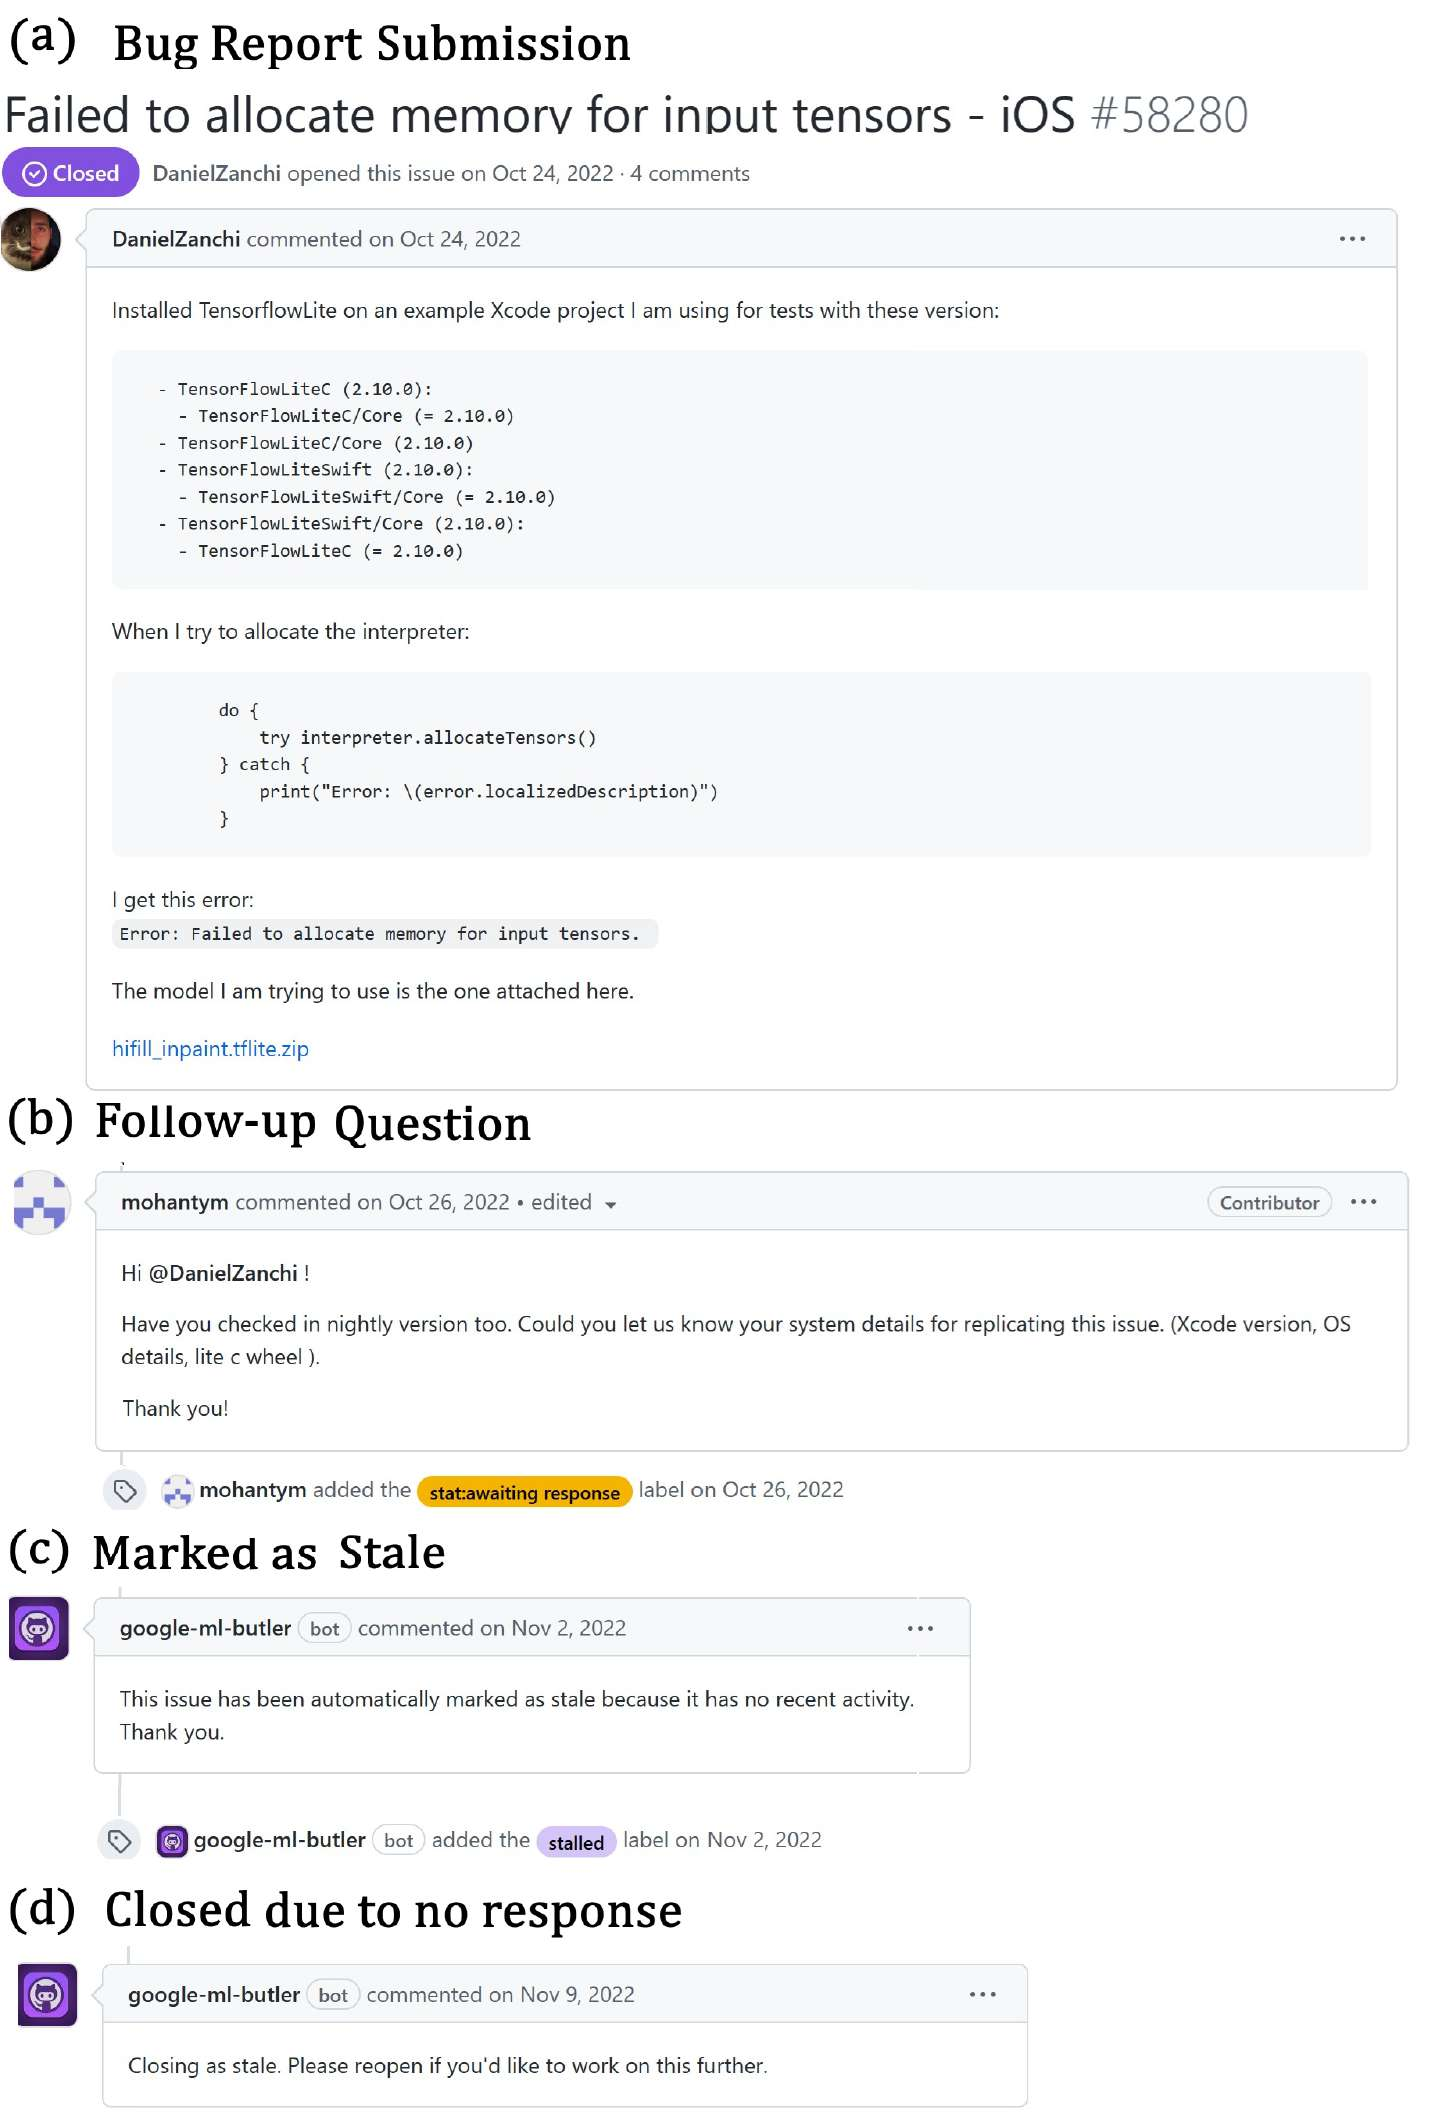
\includegraphics[ width=\textwidth, height=8.5in]{images/motivating_example_optimized.pdf}
  \caption{An example of a bug report (ID \#58280) being closed due to a lack of response to the follow-up question}
  \label{fig:motivating_example}
\end{figure}


\looseness=-1
As shown in Fig~\ref{fig:motivating_example}, without proper support in gathering missing information, software bugs either take longer to be resolved or remain unresolved and are ultimately closed. Several bugs, such as memory allocation bugs, are considered to be severe~\cite{li2006bugseverity} that significantly impact software quality. Our work --- BugMentor --- delivers meaningful answers to the follow-up questions, as shown in the answer for issue \#58280. \par

\begin{frshaded}
    % \vspace{-0.3cm}
    \begin{center}
        \textbf{Answer for issue \#58280 }
        % \label{bumentor-ans}
    \end{center}
        \noindent
        \textbf{Question:} Have you checked in nightly version too? Could you let us know your system details for replicating this issue (Xcode Version, OS details, lite c wheel)?\\
        \textbf{Generated Answer: }Adding two flags to Xcode's `Other Linker Flags' settings and modify the Podfile to use the nightly TensorFlow build, specifically `TensorFlowLiteSwift' and `TensorFlowLiteSelectTfOps'.
\end{frshaded}

\looseness=-1
We see that BugMentor was able to capture the context of the discussed problem above and provide useful suggestions. According to the bug report (Fig.~\ref{fig:motivating_example}), integrating the TensorFlow library into an Xcode project resulted in a memory allocation bug. BugMentor suggests modifying the \textit{``Other Linker Flags"} from Xcode to link the IDE to various versions of the TensorFlow library, such as \textit{TensorFlowLiteSwift} or \textit{TensorFlowLiteSelectTfOps}. It should be noted that these library versions were carefully extracted by our technique from the problem context in the bug report. Furthermore, BugMentor was able to deliver complementary information (e.g., \textit{Other Linker Flags}) that could be useful in resolving the library integration problem. The effectiveness of such an idea was further confirmed by a discussion on StackOverflow Q\&A site~\cite{linkerflags}.
% \vspace{-0.1cm}

% \vspace{-0.4cm}


\section{BugMentor: Proposed Technique} \label{Chap1:BugMentor}


\begin{figure}[htbp]
  \centering
  \rotatebox{270}{%
    \begin{minipage}{\textheight}
      \centering
      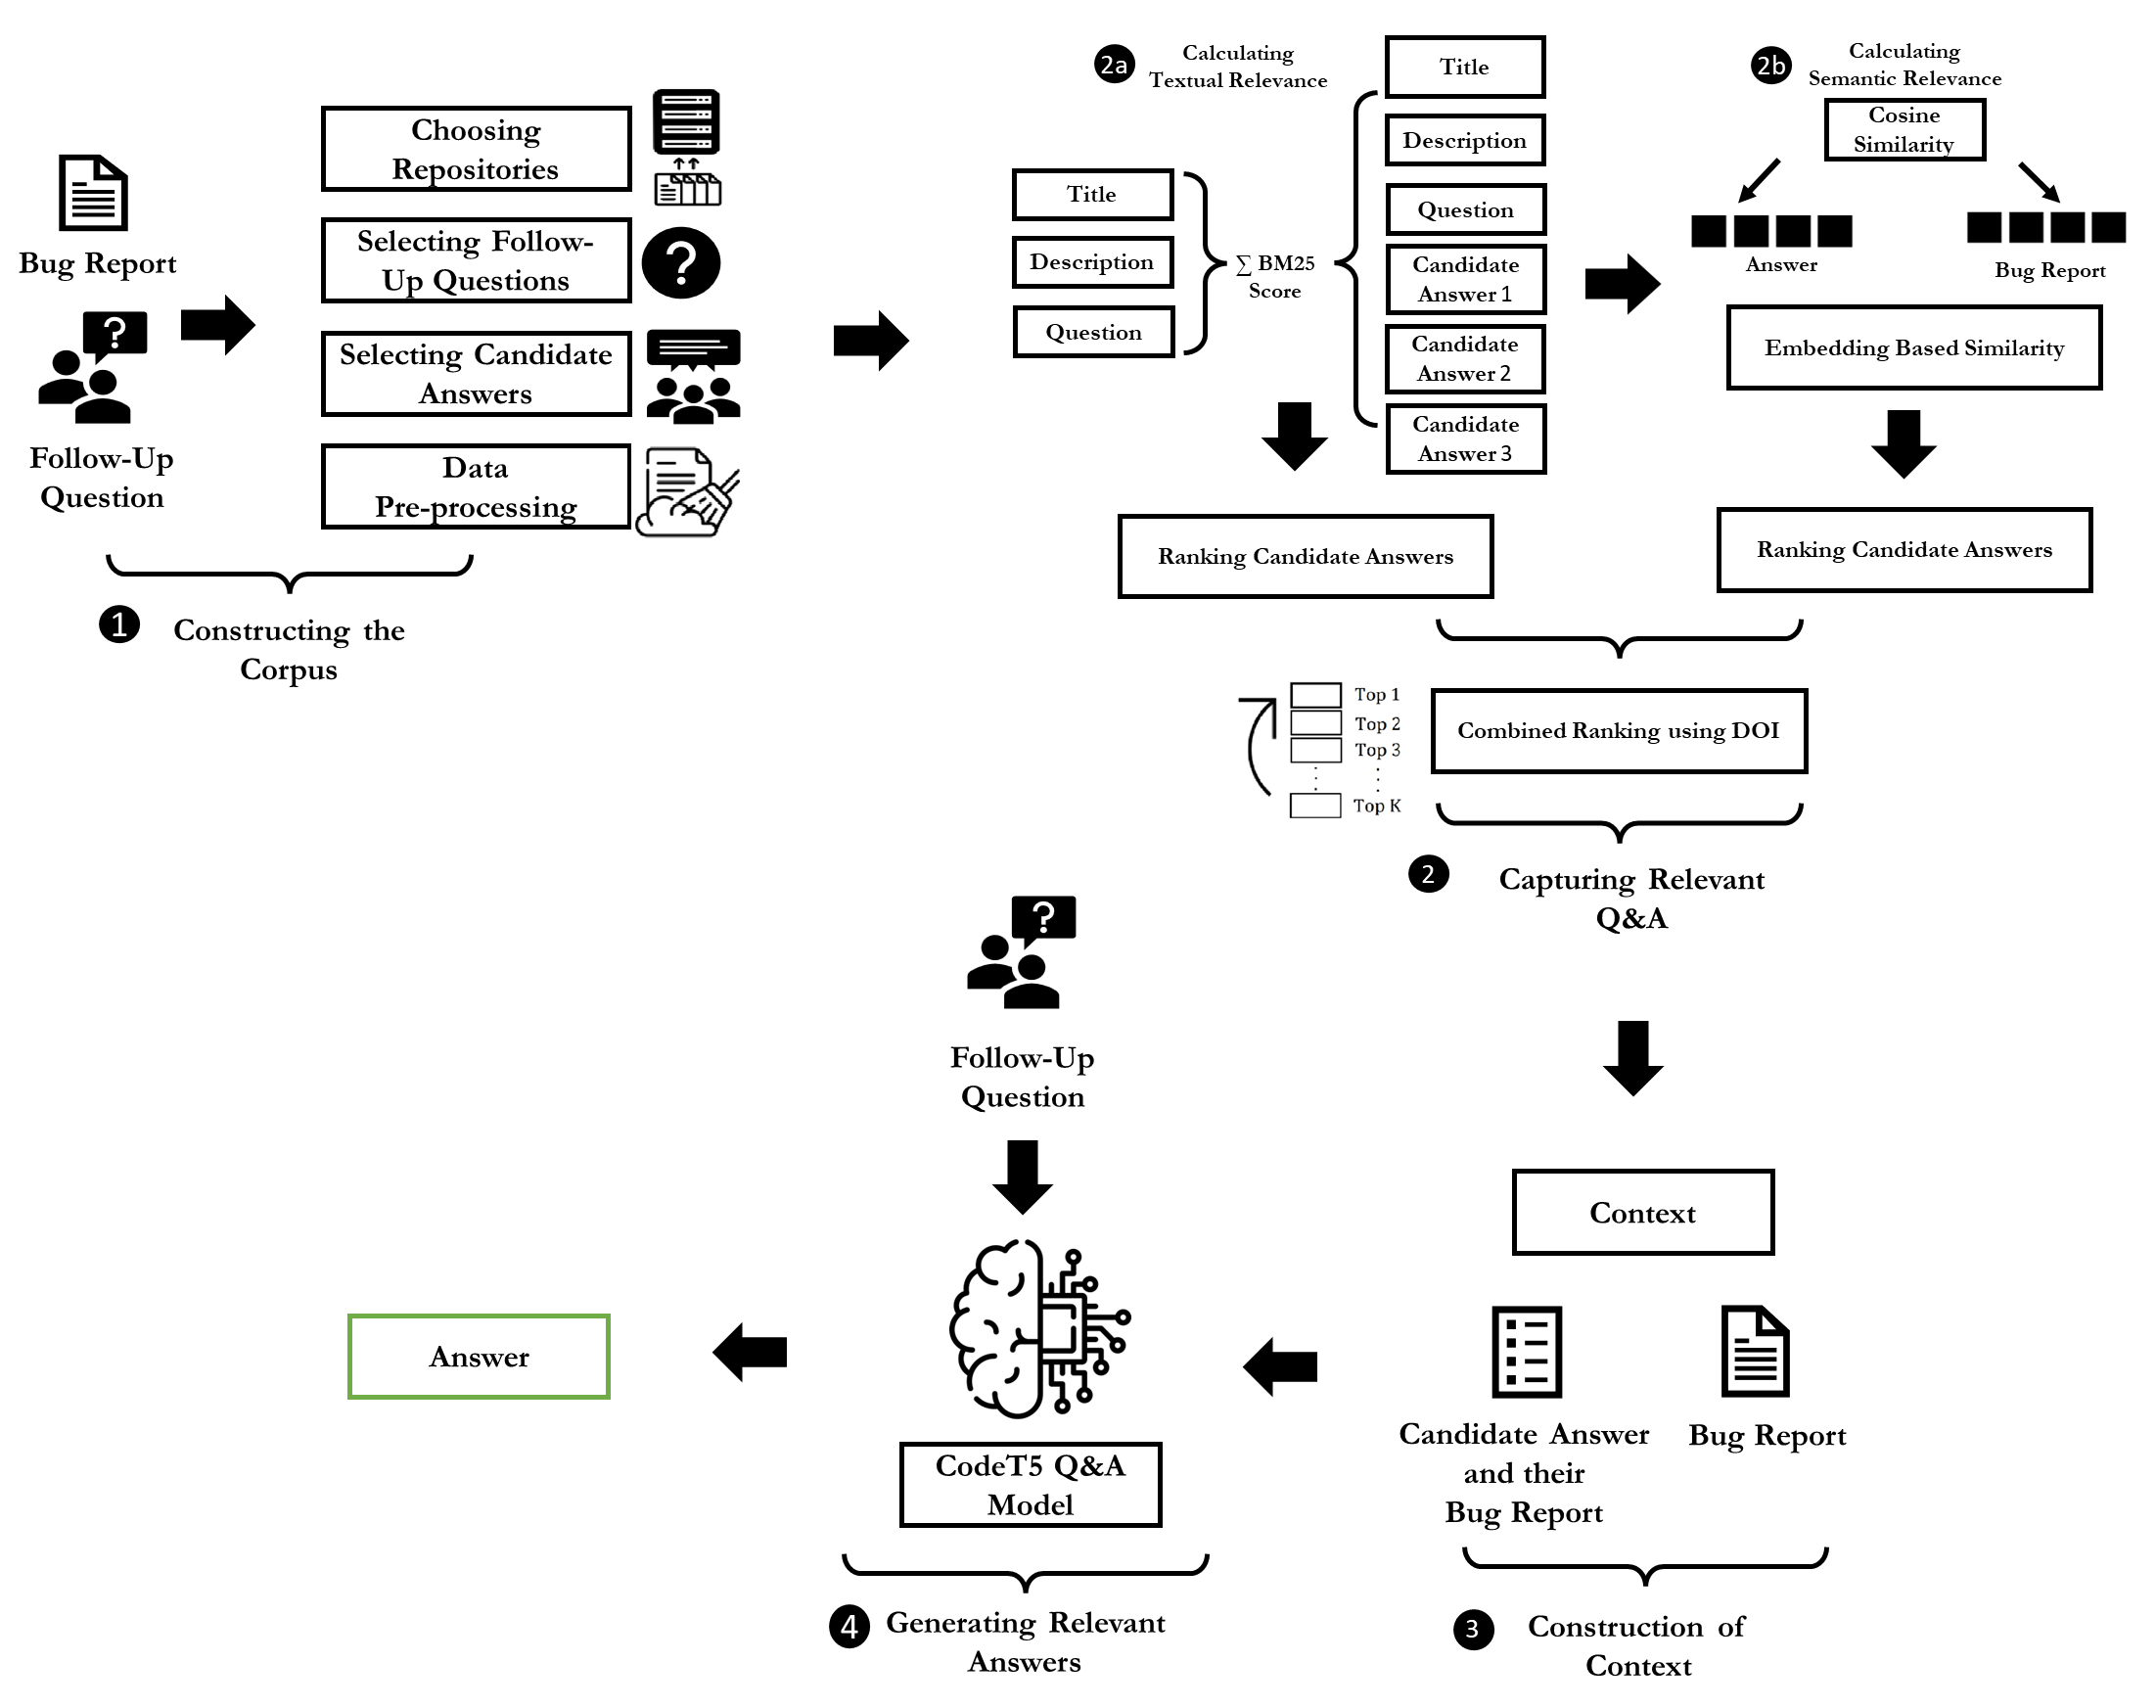
\includegraphics[width=0.9\textwidth, height=\textwidth,keepaspectratio]{images/BugMentorSchematic3.png}
      \caption{Schematic diagram of BugMentor}
      \label{fig:algo}
    \end{minipage}%
  }
\end{figure}

\looseness=-1
Fig.~\ref{fig:algo} shows the schematic diagram of our proposed technique --- BugMentor. As the input, it accepts a bug report of interest, its follow-up question, and a corpus of past bug reports with their follow-up questions and corresponding answers. As the output, our technique generates a relevant answer to the follow-up question. We discuss different steps of our technique in detail in the following sections.\par

\subsection{Constructing the Corpus}
\label{sec:corpus-construction}
\looseness=-1
We construct our corpus using past bug reports and their discussion history from 20 real-world open-source software systems on GitHub (Step 1, Fig~\ref{fig:algo}).\par


\subsubsection{\textit{Choosing the Repositories for the Corpus}}
\label{sec:proposedtechnique-repo}
To construct our corpus, we collect high-quality repositories using a semi-automated approach. We follow the approach of Imran et al. ~\cite{imran2021automatically} and choose GitHub~\cite{github} as a data source. GitHub~\cite{github} is a popular open-source platform that supports various software maintenance practices, including bug report management. We select the repositories and collect the bug reports as follows.\par

First, we select the most starred active repositories containing a minimum of 500 issues (reported as of May 2023) using GitHub's advanced search~\cite{GitHubAdvancedSearch}. We then categorize the repositories into four subsets based on their programming languages --- Python, Java, Javascript and C++ --- where each programming language had five repositories.\par

\subsubsection{\textit{Choosing the Bug Reports for the Corpus}}
\looseness=-1
From each repository, we then select the issues that were closed within the last five years. We select the issues that are labelled as ``bug", ``crash", or ``defect" to ensure that they are discussing software bugs or defects. We also select the bug reports labelled as ``needs more info" and ``stale" that were closed due to a lack of activity. We use GitHub's REST API~\cite{githubdocumentation} to collect the bug reports and their discussion history. Each of our collected bug reports consists of several fields, namely issue ID, title, bug description, bug reporter, label, creation time, and resolution time. \par

\subsubsection{\textit{Selecting Follow-up Questions}}
\label{sec:proposedtechnique-followq}
To select follow-up questions from each bug report, we first collect their issue comments using a GitHub API client~\cite{koshukeGitHubLibrary}. From each comment, we capture four different fields, namely --- comment ID, author of the comment, comment, and comment time. Following the strategy of Imran et al. ~\cite{imran2021automatically}, we collect the comments that begin with an interrogative word and end with a question mark. We use NLTK's Classifier~\cite{nltkclassifydocumentation} to identify these comments, as was applied previously~\cite{yuan2012enhancing}. We also consider comments that requested additional information using words such as ‘please’ or `can you' as valid comments. Then we select the first valid, interrogative comment that is not written by the author as our follow-up question from each bug report. We manually check up to 30 comments from each bug report to identify our follow-up questions. \par

\subsubsection{\textit{Selecting Candidate Answers}}
\label{sec:proposedtechnique-candidateans}
The next step in our corpus construction is to select candidate answers against the follow-up questions above. 
We apply three criteria to the selection of our candidate answers: (a) Candidate Answer 1 --- the first comment after the follow-up question that was not authored by the question submitter ~\cite{imran2021automatically}, (b) Candidate Answer 2 --- the first comment after the follow-up question that was authored by the bug reporter, and (c) Candidate Answer 3 --- the most similar comment to the follow-up question based on BM25 algorithm~\cite{whissell2011improving}. Finally, our corpus consisted of hundreds of bug reports where we capture the Bug ID, title, description, follow-up question and three candidate answers from each bug report.\par

\subsubsection{\textit{Data Pre-processing}}
\label{sec:proposedtechnique-datapreprocessing}
\looseness=-1
We apply standard natural language pre-processing to each bug report, follow-up question and candidate answer from our corpus. First, we remove redundant or noisy elements such as escape sequences, special characters, URLs, stack traces or images from each item~\cite{imran2021automatically}. We use appropriate regular expressions from  NLTK~\cite{NLTK}
% \footnote{\url{https://www.nltk.org/}} 
to retain the natural language text and code elements while discarding the rest. Second, we perform lemmatization on all items in our corpus. This step ensures that words are transformed to their root forms, facilitating better analysis ~\cite{pramana2022systematic}.\par

\subsection{Capturing Relevant Candidate Answers}
\label{sec:proposedtechnique-relanswer}
We then capture relevant candidate answers against each follow-up question (Step 2, Fig~\ref{fig:algo}). We use the ElasticSearch implementation~\cite{ElasticSearch}
% \footnote{\url{https://www.elastic.co/elasticsearch/}} 
of Lucene~\cite{haiduc2013automatic,moreno2015query, mccandless2010lucene}, a widely adopted search engine combining Boolean search and Vector Space Model (VSM), for our task. We employ the Okapi BM25 algorithm~\cite{kamphuis2020bm25} from the engine for similarity calculation. In particular, we calculate two BM25-based relevance scores where we adapt an existing work of Saha et al.~\cite{saha2013improving}:
\vspace{-0.21cm}
\begin{equation}\label{bluir}
\vspace{-0.25cm}
  s'\left( \vec{d},\vec{q} \right) = \sum_{r\in Q}\sum_{f\in D}s(d_{f} , q_{r})
\end{equation}
Here $q_{r}$ is a query representation, and $d_{f}$ is a field from the past bug report (e.g., title, description).\par

\begin{figure}
	% \includegraphics[width=3.6in, height = 3.5in]{Capturing_Relevant_QA.png}
 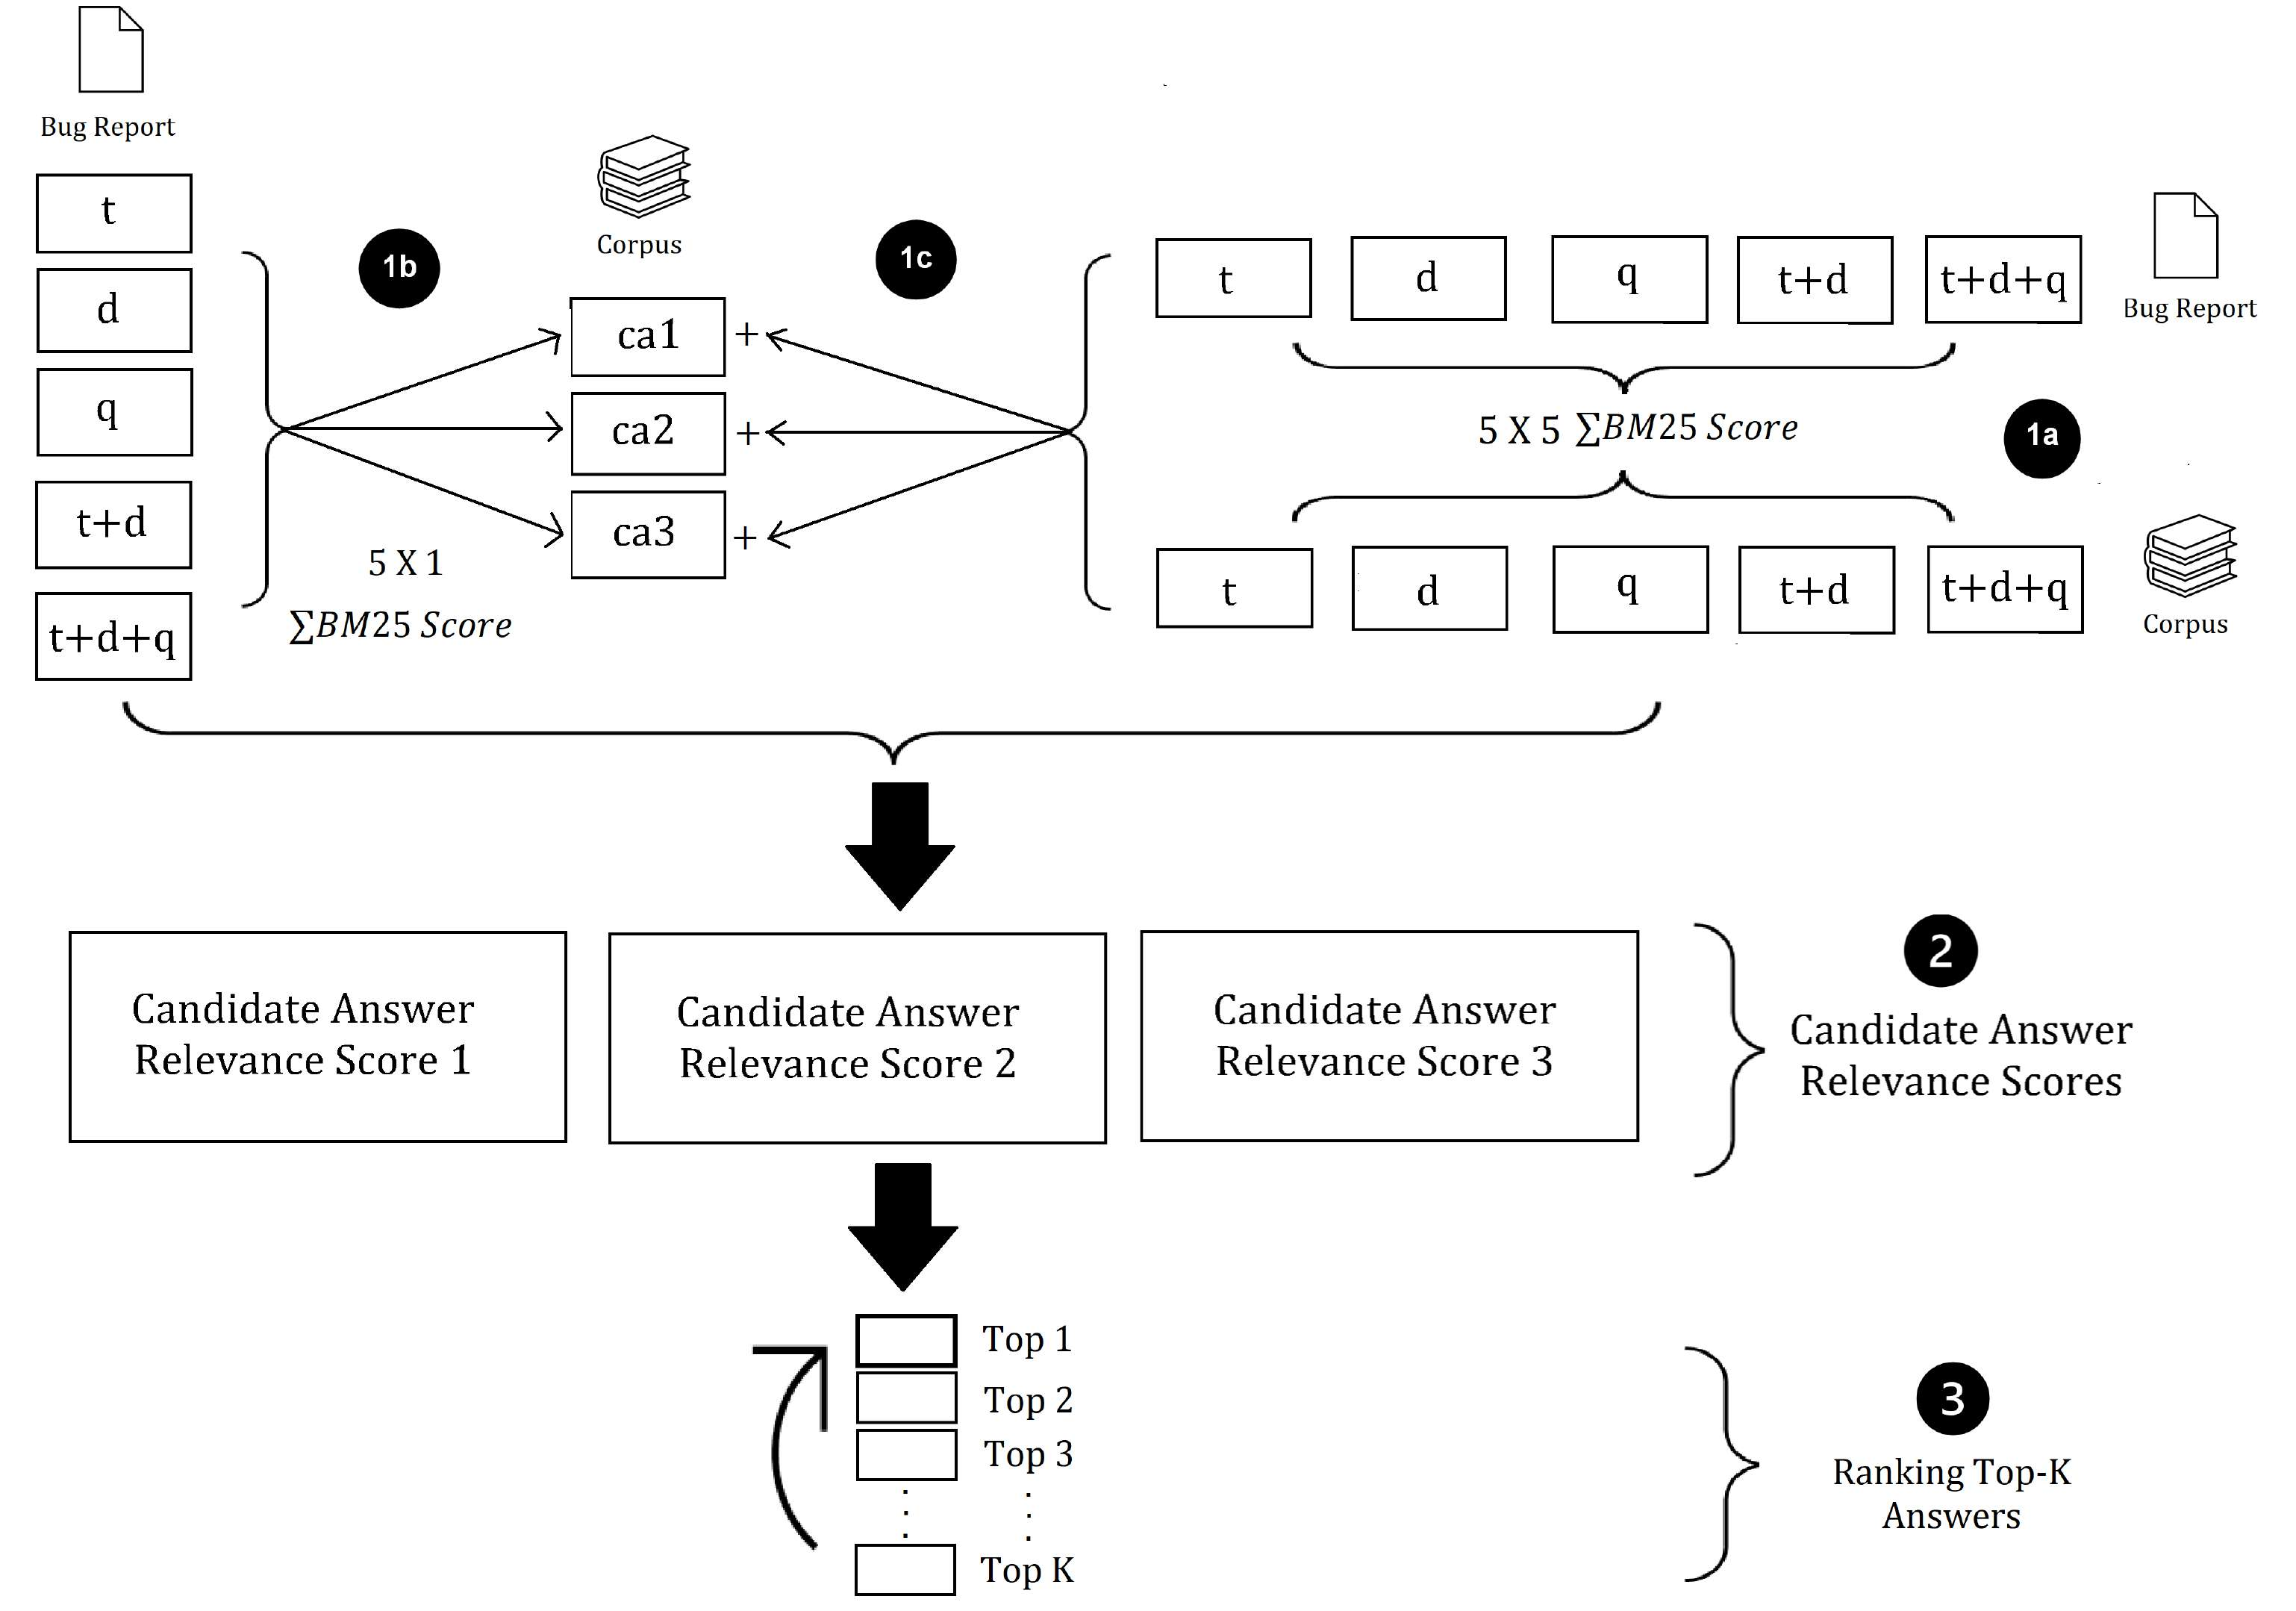
\includegraphics[width=\textwidth, height = 3.5in]{images/Capturing_Relevant_QA_Optimized.pdf}
	% \vspace{-.4cm}
	\caption{Capturing relevant answers with structured Information Retrieval}
	% \vspace{-.6cm}
	\label{fig:qa}
 	% \vspace{-.cm}
\end{figure}
% \\where t-title, d-description, q-question, ca1-candidate answer 1, ca2-candidate answer 2 and ca3-candidate answer 3
\subsubsection{Detecting Relevant Candidate Answers}
\looseness=-1
First, we capture five items from each of the given and past bug reports --- title (t), description (d), follow-up question (q), title + description (t+d), and title + description + question (t+d+q). Then we conduct 25 (5x5) similarity calculations between these bug reports using Eq~\ref{bluir}, and add all 25 similarity scores as shown in Step 1a in Fig.~\ref{fig:qa}. According to existing literature~\cite{saha2013improving}, such an element-based similarity calculation can help prevent spurious matching. This score indicates the general relevance between a given and past bug reports.\par
\looseness=-1
Second, we capture five items from the given bug report --- title (t), description (d), and follow-up question (q), title + description (t+d), and title + description + question (t+d+q) and three candidate answers (ca1, ca2, ca3) from each past bug report. Then, we conduct 5 (5x1) similarity calculations using Eq.~\ref{bluir}, for each of the three candidate answers, as shown in Step 1b, in Fig.~\ref{fig:qa}. This score indicates the relevance between the follow-up question (and its bug report) and each candidate answer.\par

While the score from Step 1a indicates a general relevance between bug reports, the score from Step 1b measures more granular relevance between the question and answer. Thus, the above two scores capture relevance from two different aspects that could be complementary to each other. We thus combine the scores from Step 1a and Step 1b to determine the relevance of each answer against the given follow-up question (and corresponding bug report) in Step 1c.\par

\subsubsection{Ranking Based on Textual Relevance}
We rank the candidate answers based on their BM25-based relevance scores calculated above (Steps 1-2, Fig.~\ref{fig:qa}). In particular, we capture the top K (e.g., 5) relevant candidate answers from the corpus against a follow-up question (Steps 3, Fig.~\ref{fig:qa}). It should be noted that these answers can come from various bug reports.\par

\subsubsection{Ranking Based on Semantic Relevance}
\looseness=-1
BM25 algorithm relies on keyword matching for relevance estimation, which could suffer from the vocabulary mismatch problem~\cite{furnas1987vocabulary}. We thus incorporate embedding-based similarity into our approach and detect the semantically relevant candidate answers. We capture word embeddings, trained by Word2Vec~\cite{church2017word2vec} on Stack Overflow~\cite{efstathiou2018word}, and calculate the cosine similarity between the embeddings of the follow-up question and that of each candidate answer. We then re-rank the answers based on their semantic relevance to the question and return the top K answers.\par

\subsubsection{Capturing the Top Relevant Answers}
\looseness=-1
We combine both BM25-based ranking and semantic relevance-based ranking using the Degree of Interest (DOI) method. Rahman et al.~\cite{rahman2016rack} use the following formulae to combine two orthogonal rankings:\par

\begin{equation}
DOI = \frac{I}{N} 
\end{equation}

\looseness=-1
Here, $I$ is the position of an answer in the ranked list and $N$ is the total number of answers. First, we calculate the DOI score of each answer within the BM25-based list and then, we calculate the DOI score within the semantic relevance-based ranked list. Then we combined the DOI scores for each answer and rank the answers based on their combined DOI score.\par

\subsection{Constructing the Context}
\looseness=-1
Generative question-answering models such as CodeT5 rely on \textit{context} to comprehensively understand the semantics or intent of a question and to generate an answer to the question~\cite{huggingfacegenerativeqa,seonwoo2020context}. We thus construct the context to enrich our follow-up question (Step 3, Fig~\ref{fig:algo}).
To construct the context, we use three items from the previous step --- one answer from the ranked list, its bug report, and the given bug report. The answer and its bug report are likely to contain additional information to compensate for the missing information in the given bug report that triggers a follow-up question. We repeat the context construction for each of the K candidate answers and send them to our CodeT5 model for final answers.\par 

\subsection{Generating Relevant Answers}
\looseness=-1
We then generate relevant answers to the follow-up question by leveraging our context above with CodeT5, a pre-trained encoder-decoder Transformer model for neural text generation. CodeT5 has been pre-trained on  8.35M methods from open-source code accompanied by documentation and adopts an encoder-decoder network to generate texts~\cite{wang2021codet5} (Step 3, Fig~\ref{fig:algo}). The model requires two components to operate, a question and its context. We provide the model with a follow-up question and its context from the previous step and capture an answer to the follow-up question from the model. For example, our technique --- BugMentor --- offers the following answer against the example question in Fig.~\ref{fig:motivating_example}.\par

\FrameSep.3em
\begin{frshaded}
\noindent	
\textbf{Generated Answer: }Adding two flags to Xcode's `Other Linker Flags' settings and modify the Podfile to use the nightly TensorFlow build, specifically `TensorFlowLiteSwift' and `TensorFlowLiteSelectTfOps'
\end{frshaded}



\section{Experiment} \label{Chap1:Experiment}
\looseness=-1
We curated a large dataset containing 30,869 bug reports and their follow-up questions from 20 subject systems and evaluate BugMentor using four appropriate metrics from relevant literature --- BLEU~\cite{papineni2002bleu}, METEOR ~\cite{banerjee2005meteor}, Semantic Similarity~\cite{haque2022semantic} and WMD~\cite{huang2016supervised}. To place our work in the literature, we also conduct an ablation study~\cite{mccandless2010lucene,wang2021codet5} and compare our technique with three baseline techniques. %abalation~\cite{mccandless2010lucene,wang2021codet5}. 
Through our experiments, we answer four research questions as follows:
\begin{enumerate}
\item[(a)] \textbf{RQ$\mathbf{_1}$}: How does our technique perform in answering follow-up questions in terms of different automatic evaluation metrics?
\item[(b)] \textbf{RQ$\mathbf{_2}$}: Can our technique outperform the existing baselines in terms of automatic evaluation metrics?
\item[(c)]\textbf{RQ$\mathbf{_3}$}: How do different components impact the overall performance of BugMentor?
\item[(d)]\textbf{RQ$\mathbf{_4}$}: How accurate, precise, useful, and concise are the answers from BugMentor?
\end{enumerate}

% \subsection{Dataset Collection}

% \subsection{Feasibility Study}
% To investigate the feasibility of our study, we manually examined 450 bug reports comprising of 30 most recent bug reports from 15 different repositories with a high number of issues and forks. Our examination focused on evaluating the quality of the follow-up questions and the received answers.\par
% During our analysis, we observed that many follow-up questions were generic in nature and existing answers to these questions were frequently present in the comments of previous bug reports, duplicate or similar bug reports. Although the answers were not completely syntactically similar, they provided additional information.\par

\subsection{Dataset Construction}\label{sec:dataset-cons}
\subsubsection{Corpus Creation}

\looseness=-1
To construct our corpus, we chose the top 20 popular projects from GitHub written in 4 different programming languages and collected 30,869 bug reports from them. We also capture a follow-up question and three candidate answers from each bug report. Finally, our corpus consisted of hundreds of bug reports where we capture the Bug ID, title, description, follow-up question and three candidate answers from each bug report. We apply standard natural language pre-processing to each item from our corpus. Please check Section~\ref{sec:corpus-construction} for further details on corpus construction.\par

\subsubsection{Ground-Truth Construction}
\label{sec:groundtruth}

\looseness=-1
To evaluate BugMentor, we first construct a randomly sampled held-out dataset (i.e., 95\% confidence level and 4.06\% error margin) containing 550 bug reports ($\sim$27 bug reports x 20 systems). We then involve six human annotators (e.g., graduate students) to determine the ground truth answers against the follow-up question from each bug report. We divided 550 bug reports into six buckets (Table~\ref{tab:interannotatoragreement}), each containing $\sim$90 bug reports, their questions, and candidate answers. Each bucket was annotated by three annotators, resulting in $\sim$270-275 bug reports per annotator. We used majority voting ~\cite{kuhrmann2017pragmatic} to determine the ground truth answers. That is, the answer having the majority of votes was chosen as the ground truth answer against a follow-up question. When the answers did not have a clear majority, i.e. for 3\% of the dataset, the three annotators engaged in discussions to resolve conflicts and determine the ground truth answer~\cite{kuhrmann2017pragmatic}. Each annotator spent $\sim$2.5-3 hours to complete the annotation. \par

\looseness=-1
We compute the Cohen's \emph{$\kappa$} for all pairs of annotators, and the result is reported in Table~\ref{tab:interannotatoragreement}. Although we use majority voting for annotation, our calculated metrics show the agreement level for each pair of annotators. We found an average of 0.46, which indicates a moderate agreement between any two annotators.\par

\begin{table*}[!t]
\centering
\caption{Inter-annotator Agreement}
\label{tab:interannotatoragreement}
\resizebox{\textwidth}{!}{
\begin{tabular}{|cc|cc|cc|cc|cc|cc|}
\hline
\multicolumn{2}{|c|}{\textbf{Bucket 1}}     & \multicolumn{2}{c|}{\textbf{Bucket 2}}     & \multicolumn{2}{c|}{\textbf{Bucket 3}}     & \multicolumn{2}{c|}{\textbf{Bucket 4}}     & \multicolumn{2}{c|}{\textbf{Bucket 5}}     & \multicolumn{2}{c|}{\textbf{Bucket 6}}     \\ \hline
\multicolumn{1}{|c|}{\textbf{Pairs}} & \textbf{$\kappa$}    & \multicolumn{1}{c|}{\textbf{Pairs}} & \textbf{$\kappa$}    & \multicolumn{1}{c|}{\textbf{Pairs}} & \textbf{$\kappa$}    & \multicolumn{1}{c|}{\textbf{Pairs}} & \textbf{$\kappa$}    & \multicolumn{1}{c|}{\textbf{Pairs}} & \textbf{$\kappa$}    & \multicolumn{1}{c|}{\textbf{Pairs}} & \textbf{$\kappa$}    \\ \hline \hline
\multicolumn{1}{|c|}{A1 \& A2}       & 0.72 & \multicolumn{1}{c|}{A2 \& A3}       & 0.58 & \multicolumn{1}{c|}{A3 \& A4}       & 0.44 & \multicolumn{1}{c|}{A4 \& A5}       & 0.66 & \multicolumn{1}{c|}{A5 \& A6}       & 0.49 & \multicolumn{1}{c|}{A1 \& A2}       & 0.41 \\ \hline
\multicolumn{1}{|c|}{A2 \& A3}       & 0.24 & \multicolumn{1}{c|}{A3 \& A4}       & 0.43 & \multicolumn{1}{c|}{A4 \& A5}       & 0.53 & \multicolumn{1}{c|}{A5 \& A6}       & 0.40 & \multicolumn{1}{c|}{A1 \& A5}       & 0.44 & \multicolumn{1}{c|}{A2 \& A6}       & 0.29 \\ \hline
\multicolumn{1}{|c|}{A3 \& A1}       & 0.39 & \multicolumn{1}{c|}{A4 \& A2}       & 0.58 & \multicolumn{1}{c|}{A5 \& A3}       & 0.65 & \multicolumn{1}{c|}{A6 \& A4}       & 0.27 & \multicolumn{1}{c|}{A6 \& A1}       & 0.49 & \multicolumn{1}{c|}{A6 \& A1}       & 0.40 \\ \hline
\end{tabular}}
\end{table*}


\subsection{Evaluation Metrics}

\looseness=-1
To evaluate BugMentor's answers against the ground truth, we use four relevant metrics from literature --- BLEU Score~\cite{papineni2002bleu}, METEOR Score~\cite{banerjee2005meteor}, Word Mover's Distance~\cite{huang2016supervised} and Semantic Similarity metric~\cite{haque2022semantic}. They are defined as follows:\par


\subsubsection{\emph{\textit{1) BLEU --- Bi-Lingual Evaluation of Understudy: }}}
\looseness=-1
\acrshort{BLEU} score is a commonly used metric for evaluating translation~\cite{papineni2002bleu}, which has found application in many software engineering tasks (e.g., comment generation \cite{hu2020deep}). It compares a candidate text to a reference text and determines how similar they are based on the matching of their n-grams. The \acrshort{BLEU} score is calculated as follows:\par

\begin{equation}
BLEU = BP \cdot exp \left ( \sum_{n=1}^{N}w_{n}log(p_{n}) \right )
\end{equation}

where $N$ is the maximum n-gram order, $w\textsubscript{n}$ is the weight assigned to the n-gram order, $BP$ is the brevity penalty - a factor that penalizes the \acrshort{BLEU} score when the candidate text is shorter than the reference text and $p\textsubscript{n}$ is the modified n-gram precision, which measures the ratio of the overlapping n-grams (between the candidate text and the reference text), and the total number of n-grams in the candidate text.\par



\subsubsection{\emph{ \textit{2) METEOR --- Metric for Evaluation of Translation with Explicit ORdering: }}}
\looseness=-1
The \acrshort{METEOR} score is a metric for evaluating the quality of machine translation output based on both lexical and syntactic information~\cite{banerjee2005meteor}. It measures the similarity between a candidate text and the reference text by sequentially applying exact match, stemmed match and wordnet-based synonym match between the texts. 


\subsubsection{\emph{\textit{3) WMD --- Word Mover's Distance: }}}
\looseness=-1
\acrshort{WMD} ~\cite{huang2016supervised} is a similarity measure between two texts based on the meaning or relationships between their words. It is the minimum cost to transform one text into another by calculating the  Euclidean distance between their word embeddings. 



\subsubsection{\emph{\textit{4) SS --- Semantic Similarity: }}}

\looseness=-1
In a recent work, Haque et al.~\cite{haque2022semantic} investigate which metric reflects human assessment of similarity the best. They suggest that Sentence-BERT~\cite{reimers2019sentence} provides semantically meaningful sentence embeddings. Thus when a candidate text is compared with the reference text based on these embeddings using cosine-similarity, it has the highest correlation with human-evaluated similarity. Semantic similarity is computed as follows:

\begin{equation}
SemSim(ref, gen) = \cos(\text{sbert}(ref), \text{sbert}(gen))  
\end{equation}

where $sbert(ref)$, $sbert(gen)$ are the numerical representations from Sentence-BERT for the reference text and generated text respectively.\par

\section{Evaluation of BugMentor} \label{Chap1:Evaluation}
\label{sec:evaluation}


\subsection{Answering RQ$\mathbf{_1}$ --- How does our technique perform in answering follow-up questions in terms of different automatic evaluation metrics?}

In this experiment, we analyze the performance of BugMentor using four different evaluation metrics - \acrshort{BLEU} score~\cite{papineni2002bleu}, \acrlong{Semantic Similarity} ~\cite{haque2022semantic}, \acrshort{METEOR}~\cite{banerjee2005meteor} and WMD~\cite{huang2016supervised}. We divide our held-out dataset into four subsets based on their corresponding programming languages and report the results for each subset. Table~\ref{tab:bugmentorcontext2} shows the performance details of BugMentor in various settings - within the project and cross-project. It should be noted that a higher value for \acrshort{BLEU}, \acrshort{METEOR}, and \acrlong{Semantic Similarity} and a lower value for \acrshort{WMD} metrics are desirable in our experiments.\par

% hybrid - context 2
\renewcommand{\arraystretch}{1.1}
\begin{table*}[!ht]
\centering
\caption{Performance of BugMentor}
\label{tab:bugmentorcontext2}
\resizebox{0.8\textwidth}{!}{%
\begin{tabular}{|ccccccc|}
\hline
\multicolumn{1}{|c|}{\textbf{Metrics}} & \multicolumn{1}{c|}{\textbf{Top K}} & \multicolumn{1}{c|}{\textbf{Python}} & \multicolumn{1}{c|}{\textbf{Java}} & \multicolumn{1}{c|}{\textbf{JavaScript}} & \multicolumn{1}{c|}{\textbf{C++}} & \textbf{Whole Dataset} \\ \hline \hline
\multicolumn{7}{|c|}{\textbf{Within Project}} \\ \hline \hline
\multicolumn{1}{|c|}{\multirow{3}{*}{\textbf{BLEU $\uparrow$}}} & \multicolumn{1}{c|}{Top 1} & \multicolumn{1}{c|}{26.20} & \multicolumn{1}{c|}{22.36} & \multicolumn{1}{c|}{26.06} & \multicolumn{1}{c|}{25.73} & 24.47 \\ \cline{2-7} 
\multicolumn{1}{|c|}{} & \multicolumn{1}{c|}{Top 3} & \multicolumn{1}{c|}{29.25} & \multicolumn{1}{c|}{32.70} & \multicolumn{1}{c|}{31.76} & \multicolumn{1}{c|}{28.03} & 28.90 \\ \cline{2-7} 
\multicolumn{1}{|c|}{} & \multicolumn{1}{c|}{Top 5} & \multicolumn{1}{c|}{34.12} & \multicolumn{1}{c|}{33.82} & \multicolumn{1}{c|}{32.38} & \multicolumn{1}{c|}{30.25} & 31.94 \\ \hline
\multicolumn{1}{|c|}{\multirow{3}{*}{\textbf{METEOR $\uparrow$}}} & \multicolumn{1}{c|}{Top 1} & \multicolumn{1}{c|}{0.14} & \multicolumn{1}{c|}{0.24} & \multicolumn{1}{c|}{0.30} & \multicolumn{1}{c|}{0.21} & 0.24 \\ \cline{2-7} 
\multicolumn{1}{|c|}{} & \multicolumn{1}{c|}{Top 3} & \multicolumn{1}{c|}{0.23} & \multicolumn{1}{c|}{0.26} & \multicolumn{1}{c|}{0.34} & \multicolumn{1}{c|}{0.26} & 0.36 \\ \cline{2-7} 
\multicolumn{1}{|c|}{} & \multicolumn{1}{c|}{Top 5} & \multicolumn{1}{c|}{0.29} & \multicolumn{1}{c|}{0.57} & \multicolumn{1}{c|}{0.36} & \multicolumn{1}{c|}{0.29} & 0.42 \\ \hline
\multicolumn{1}{|c|}{\multirow{3}{*}{\textbf{SS $\uparrow$}}} & \multicolumn{1}{c|}{Top 1} & \multicolumn{1}{c|}{43.20} & \multicolumn{1}{c|}{42.90} & \multicolumn{1}{c|}{46.30} & \multicolumn{1}{c|}{46.13} & 50.63 \\ \cline{2-7} 
\multicolumn{1}{|c|}{} & \multicolumn{1}{c|}{Top 3} & \multicolumn{1}{c|}{58.80} & \multicolumn{1}{c|}{42.90} & \multicolumn{1}{c|}{45.50} & \multicolumn{1}{c|}{54.30} & 53.49 \\ \cline{2-7} 
\multicolumn{1}{|c|}{} & \multicolumn{1}{c|}{Top 5} & \multicolumn{1}{c|}{64.50} & \multicolumn{1}{c|}{54.70} & \multicolumn{1}{c|}{54.20} & \multicolumn{1}{c|}{56.10} & 57.01 \\ \hline
\multicolumn{1}{|c|}{\multirow{3}{*}{\textbf{WMD $\downarrow$}}} & \multicolumn{1}{c|}{Top 1} & \multicolumn{1}{c|}{5.09} & \multicolumn{1}{c|}{4.97} & \multicolumn{1}{c|}{4.91} & \multicolumn{1}{c|}{5.35} & 4.18 \\ \cline{2-7} 
\multicolumn{1}{|c|}{} & \multicolumn{1}{c|}{Top 3} & \multicolumn{1}{c|}{4.89} & \multicolumn{1}{c|}{4.64} & \multicolumn{1}{c|}{4.75} & \multicolumn{1}{c|}{4.93} & 3.80 \\ \cline{2-7} 
\multicolumn{1}{|c|}{} & \multicolumn{1}{c|}{Top 5} & \multicolumn{1}{c|}{4.82} & \multicolumn{1}{c|}{3.27} & \multicolumn{1}{c|}{4.29} & \multicolumn{1}{c|}{4.56} & 3.65 \\ \hline \hline
\multicolumn{7}{|c|}{\textbf{Cross Project}} \\ \hline  \hline
\multicolumn{1}{|c|}{\multirow{3}{*}{\textbf{BLEU $\uparrow$}}} & \multicolumn{1}{c|}{Top 1} & \multicolumn{1}{c|}{16.71} & \multicolumn{1}{c|}{14.24} & \multicolumn{1}{c|}{12.36} & \multicolumn{1}{c|}{16.03} & 14.84 \\ \cline{2-7} 
\multicolumn{1}{|c|}{} & \multicolumn{1}{c|}{Top 3} & \multicolumn{1}{c|}{20.52} & \multicolumn{1}{c|}{15.12} & \multicolumn{1}{c|}{16.99} & \multicolumn{1}{c|}{18.97} & 17.90 \\ \cline{2-7} 
\multicolumn{1}{|c|}{} & \multicolumn{1}{c|}{Top 5} & \multicolumn{1}{c|}{21.86} & \multicolumn{1}{c|}{17.70} & \multicolumn{1}{c|}{19.30} & \multicolumn{1}{c|}{19.92} & 19.70 \\ \hline
\multicolumn{1}{|c|}{\multirow{3}{*}{\textbf{METEOR $\uparrow$}}} & \multicolumn{1}{c|}{Top 1} & \multicolumn{1}{c|}{0.12} & \multicolumn{1}{c|}{0.13} & \multicolumn{1}{c|}{0.11} & \multicolumn{1}{c|}{0.09} & 0.11 \\ \cline{2-7} 
\multicolumn{1}{|c|}{} & \multicolumn{1}{c|}{Top 3} & \multicolumn{1}{c|}{0.14} & \multicolumn{1}{c|}{0.16} & \multicolumn{1}{c|}{0.13} & \multicolumn{1}{c|}{0.11} & 0.14 \\ \cline{2-7} 
\multicolumn{1}{|c|}{} & \multicolumn{1}{c|}{Top 5} & \multicolumn{1}{c|}{0.15} & \multicolumn{1}{c|}{0.19} & \multicolumn{1}{c|}{0.14} & \multicolumn{1}{c|}{0.12} & 0.15 \\ \hline
\multicolumn{1}{|c|}{\multirow{3}{*}{\textbf{SS $\uparrow$}}} & \multicolumn{1}{c|}{Top 1} & \multicolumn{1}{c|}{26.80} & \multicolumn{1}{c|}{26.23} & \multicolumn{1}{c|}{27.76} & \multicolumn{1}{c|}{27.30} & 27.02 \\ \cline{2-7} 
\multicolumn{1}{|c|}{} & \multicolumn{1}{c|}{Top 3} & \multicolumn{1}{c|}{29.15} & \multicolumn{1}{c|}{29.52} & \multicolumn{1}{c|}{29.75} & \multicolumn{1}{c|}{29.27} & 29.42 \\ \cline{2-7} 
\multicolumn{1}{|c|}{} & \multicolumn{1}{c|}{Top 5} & \multicolumn{1}{c|}{31.89} & \multicolumn{1}{c|}{31.80} & \multicolumn{1}{c|}{30.93} & \multicolumn{1}{c|}{30.75} & 31.34 \\ \hline
\multicolumn{1}{|c|}{\multirow{3}{*}{\textbf{WMD $\downarrow$}}} & \multicolumn{1}{c|}{Top 1} & \multicolumn{1}{c|}{5.23} & \multicolumn{1}{c|}{5.62} & \multicolumn{1}{c|}{5.10} & \multicolumn{1}{c|}{5.43} & 5.34 \\ \cline{2-7} 
\multicolumn{1}{|c|}{} & \multicolumn{1}{c|}{Top 3} & \multicolumn{1}{c|}{5.02} & \multicolumn{1}{c|}{5.64} & \multicolumn{1}{c|}{5.01} & \multicolumn{1}{c|}{5.38} & 5.26 \\ \cline{2-7} 
\multicolumn{1}{|c|}{} & \multicolumn{1}{c|}{Top 5} & \multicolumn{1}{c|}{4.87} & \multicolumn{1}{c|}{5.68} & \multicolumn{1}{c|}{4.98} & \multicolumn{1}{c|}{5.36} & 5.22 \\ \hline
\end{tabular}%
}
\end{table*}

\looseness=-1
BugMentor achieves an average BLEU Score of 24.47 for Top 1 answer, and a maximum of 31.94 for Top 5 answers when our whole dataset is considered. In the case of cross-project setting, these scores drop to 14.84 and 19.70, respectively. However, our technique achieves a maximum of 26.20 for the Top 1, 32.7 for Top 3 and 34.12 for Top 5 answers across all four subsets. These BLEU scores indicate that our generated answers are \textit{understandable} and \textit{good} according to Google’s AutoML Translation documentation~\cite{automldoc}. This also shows that the answers generated by BugMentor have a significant overlap with the ground truth in terms of words and word order. However, BLEU score primarily focuses on capturing the precision of an answer against the ground truth. Hence we also evaluate our answers using the METEOR score, where recall is captured by taking into account additional information such as synonyms, word forms, and sentence structure ~\cite{banerjee2005meteor}.\par

As shown in Table~\ref{tab:bugmentorcontext2}, BugMentor achieves an average METEOR score of 0.24 for Top 1 answer, and a maximum of 0.42 for Top 5 answers against the whole dataset, which are considered to be reasonable~\cite{agarwal2008meteor}. In cross-project setting, our technique achieves an average METEOR score of 0.11 for Top 1 answer, and a maximum of 0.15 for Top 5 answers. It achieves a maximum of 0.30 for Top 1, 0.34 for Top 3, and 0.57 for Top 5 answers across four subsets. This shows that BugMentor was able to produce a significant part of the ground truth texts in the generated answers. However, since BLEU and METEOR scores rely on keyword matching between a generated answer and the ground truth answer, they may not capture the semantic relevance between them. Hence we also evaluate our technique using WMD~\cite{huang2016supervised} and Semantic Similarity~\cite{haque2022semantic}. They also have been shown to correlate better with human judgement of relevance ~\cite{papineni2002bleu, kusner2015word}. \par

\looseness=-1
In Table~\ref{tab:bugmentorcontext2}, we find that BugMentor achieves an average WMD of 4.18 for Top 1 answer, and a minimum of 3.65 for Top 5 answers, when the whole dataset is considered. In cross-project setting, our technique achieves an average WMD of 5.34 for Top 1 answer, and a minimum of 5.22 for Top 5 answers. These distance scores show that BugMentor was able to generate answers semantically similar to the ground truth and were worded closely to the ground truth. However, WMD may not be sufficient to reflect the importance and context of words in a sentence ~\cite{kusner2015word,sato2022re}. We thus also evaluate our answers using semantic similarity against the ground truth. The metric is appropriate when there may not be any syntactic overlap between the answers, which is a common phenomenon in question answering, according to existing literature ~\cite{yao2013answer,severyn2015learning}.\par

\looseness=-1
From Table ~\ref{tab:bugmentorcontext2}, we also find that the answers from BugMentor have an average Semantic Similarity score of  50.63\% for Top 1 answer, and a maximum of 57.01\% for Top 5 answers when the whole dataset is considered. It achieves an average Semantic Similarity score of 27.02\% for Top 1 answer, and a maximum 31.34\% for Top 5 answer in cross-project setting. BugMentor achieves a maximum of 46.13\% for Top 1, and a maximum of 64.5\% for Top 5 answers when all subsets are considered. All these numbers indicate a high similarity in meaning and content between BugMentor's answers and the ground truth.\par


\FrameSep.3em
\begin{frshaded}
	\noindent
	\textbf{Summary of RQ$\mathbf{_1}$:} BugMentor can generate relevant answers to follow-up questions that are \textit{understandable} to \textit{good} according to Google's Standard and achieves an average BLEU score of 31.94. Its answers also have a high semantic overlap with the ground truth answers and thus achieve an average semantic similarity score of 57\%.
\end{frshaded}

\subsection{Answering RQ$\mathbf{_2}$ --- Can our technique outperform the existing baselines in terms of automatic evaluation metrics?}\label{results:rq2}

To the best of our knowledge, there exists no work that can offer relevant answers to follow-up questions from bug reports. However, Lucene~\cite{mccandless2010lucene} is a popular IR-based tool that has been used to recommend answers in the programming Q\&A site ~\cite{Atwood_2017,ponzanelli2013leveraging}.
CodeT5~\cite{wang2021codet5} is a large language model for generating answers to questions. AnswerBot~\cite{xu2017answerbot} can synthesize
answers for technical, non-factoid questions on StackOverflow. We thus consider them as our baselines for the comparison. We call them Baseline$_{Lucene}$, Baseline$_{CodeT5}$ and AnswerBot, respectively in this experiment. We evaluate the answers from all three baselines against the ground truth using four evaluation metrics. Tables~\ref{tab:baselinecomparison1} and ~\ref{tab:baselinecomparison2} show the comparison details between BugMentor and these baseline techniques.\par

\begin{table*}[!ht]
\centering
\caption{Comparison of BugMentor with Baseline$_{Lucene}$ and Answerbot}
\label{tab:baselinecomparison1}
\resizebox{0.7\textwidth}{!}{%
    \begin{tabular}{|ccccc|}
    \hline
    \multicolumn{1}{|c|}{\textbf{Metrics}} & \multicolumn{1}{c|}{\textbf{Top K}} & \multicolumn{1}{c|}{\textbf{AnswerBot}} & \multicolumn{1}{c|}{\textbf{Baseline$_{Lucene}$}} & \textbf{BugMentor} \\ \hline \hline
    \multicolumn{1}{|c|}{\multirow{3}{*}{\textbf{BLEU $\uparrow$}}} & \multicolumn{1}{c|}{Top 1} & \multicolumn{1}{c|}{4.31} & \multicolumn{1}{c|}{8.60} & \textbf{24.47} \\ \cline{2-5} 
    \multicolumn{1}{|c|}{} & \multicolumn{1}{c|}{Top 3} & \multicolumn{1}{c|}{6.71} & \multicolumn{1}{c|}{10.54} & \textbf{28.9} \\ \cline{2-5} 
    \multicolumn{1}{|c|}{} & \multicolumn{1}{c|}{Top 5} & \multicolumn{1}{c|}{4.24} & \multicolumn{1}{c|}{14.31} & \textbf{31.94} \\ \hline
    \multicolumn{1}{|c|}{\multirow{3}{*}{\textbf{METEOR $\uparrow$}}} & \multicolumn{1}{c|}{Top 1} & \multicolumn{1}{c|}{0.05} & \multicolumn{1}{c|}{0.18} & \textbf{0.24} \\ \cline{2-5} 
    \multicolumn{1}{|c|}{} & \multicolumn{1}{c|}{Top 3} & \multicolumn{1}{c|}{0.12} & \multicolumn{1}{c|}{0.19} & \textbf{0.36} \\ \cline{2-5} 
    \multicolumn{1}{|c|}{} & \multicolumn{1}{c|}{Top 5} & \multicolumn{1}{c|}{0.07} & \multicolumn{1}{c|}{0.21} & \textbf{0.42} \\ \hline
    \multicolumn{1}{|c|}{\multirow{3}{*}{\textbf{SS $\uparrow$}}} & \multicolumn{1}{c|}{Top 1} & \multicolumn{1}{c|}{36.47} & \multicolumn{1}{c|}{42.75} & \textbf{50.63} \\ \cline{2-5} 
    \multicolumn{1}{|c|}{} & \multicolumn{1}{c|}{Top 3} & \multicolumn{1}{c|}{47.69} & \multicolumn{1}{c|}{45.45} & \textbf{53.49} \\ \cline{2-5} 
    \multicolumn{1}{|c|}{} & \multicolumn{1}{c|}{Top 5} & \multicolumn{1}{c|}{47.69} & \multicolumn{1}{c|}{48.78} & \textbf{57.01} \\ \hline
    \multicolumn{1}{|c|}{\multirow{3}{*}{\textbf{WMD $\downarrow$}}} & \multicolumn{1}{c|}{Top 1} & \multicolumn{1}{c|}{5.7} & \multicolumn{1}{c|}{4.55} & \textbf{4.18} \\ \cline{2-5} 
    \multicolumn{1}{|c|}{} & \multicolumn{1}{c|}{Top 3} & \multicolumn{1}{c|}{4.81} & \multicolumn{1}{c|}{4.46} & \textbf{3.80} \\ \cline{2-5} 
    \multicolumn{1}{|c|}{} & \multicolumn{1}{c|}{Top 5} & \multicolumn{1}{c|}{5.01} & \multicolumn{1}{c|}{4.37} & \textbf{3.65} \\ \hline
    \end{tabular}}
\vspace{1cm} 
    \caption{Comparison of BugMentor with Baseline$_{CodeT5}$}
    \label{tab:baselinecomparison2}
    \resizebox{0.6\textwidth}{!}{%
    \begin{tabular}{|cccc|}
    \hline
    \multicolumn{1}{|c|}{\textbf{Metrics}} & \multicolumn{1}{c|}{\textbf{Top K}} & \multicolumn{1}{c|}{\textbf{Baseline$_{CodeT5}$}} & \textbf{BugMentor} \\ \hline
    \multicolumn{1}{|c|}{\textbf{BLEU $\uparrow$}} & \multicolumn{1}{c|}{\multirow{4}{*}{Top 1}} & \multicolumn{1}{c|}{2.4} & \textbf{24.47} \\ \cline{1-1} \cline{3-4} 
    \multicolumn{1}{|c|}{\textbf{METEOR $\uparrow$}} & \multicolumn{1}{c|}{} & \multicolumn{1}{c|}{0.04} & \textbf{0.24} \\ \cline{1-1} \cline{3-4} 
    \multicolumn{1}{|c|}{\textbf{SS $\uparrow$}} & \multicolumn{1}{c|}{} & \multicolumn{1}{c|}{11.01} & \textbf{50.63} \\ \cline{1-1} \cline{3-4} 
    \multicolumn{1}{|c|}{\textbf{WMD $\downarrow$}} & \multicolumn{1}{c|}{} & \multicolumn{1}{c|}{7.32} & \textbf{4.18} \\ \hline
    \end{tabular}}
\end{table*}

\looseness=-1
To implement Baseline$_{Lucene}$, we provide a follow-up question as the \emph{query} and all candidate answers as the \emph{corpus} to the Lucene tool. Then we collect the top K answers from the tool by executing the query for our evaluation. Baseline$_{Lucene}$ achieves a BLEU score of 8.60, METEOR score of 0.18, Semantic Similarity of 42.75 and WMD of 4.55. On the other hand, BugMentor achieves a BLEU score of 24.47, METEOR score of 0.24, Semantic Similarity of 50.63 and WMD of 4.18. Thus, our technique outperforms the baseline in all four metrics.\par


\looseness=-1
To implement Baseline$_{CodeT5}$, we provide a follow-up question as the \emph{query} and its corresponding bug report as \emph{context} to the CodeT5 model, which generates an answer. We observe that Baseline$_{CodeT5}$ performs significantly poorly when compared to BugMentor and  Baseline$_{Lucene}$. For example, Baseline$_{CodeT5}$ achieves a BLEU score of 2.4, METEOR score of 0.04, Semantic Similarity of 11.01 and WMD of 7.32, which are 42\%-90\% lower than the corresponding measures from BugMentor.


\looseness=-1
To implement AnswerBot, we use the replication package provided by the authors~\cite{xu2017answerbot, maxxbw54}. We provide a follow-up question as the \emph{query} and all bug reports along with their candidate answers as the \emph{corpus}. We observe that AnswerBot performs significantly poorly when compared to BugMentor and  Baseline$_{Lucene}$. For example, AnswerBot achieves a maximum BLEU score of 6.71, METEOR score of 0.12, Semantic Similarity of 47.69 and a minimum WMD of 4.81, which are lower than the corresponding measures from BugMentor.\par


\looseness=-1
We also perform Mann-Whitney Wilcoxon test~\cite{cuzick1985wilcoxon} to check if the performance of Baseline$_{Lucene}$, Baseline$_{CodeT5}$, AnswerBot are significantly lower than that of BugMentor using BonFerroni Correction~\cite{weisstein2004bonferroni}. We find that BugMentor performs significantly higher than Baseline$_{Lucene}$ and AnswerBot, i.e., p-value $=$ 0.010$<$0.016 in terms of all four metrics.\par

Besides the comparison with traditional baselines, it is important to consider the other the competitive landscape, particularly with the emergence of popular Language Model-based approaches (LLMs) such as ChatGPT. Upon conducting a limited qualitative analysis, we observe that while ChatGPT exhibit a profound understanding of the bug report context, they fall short in providing answers to follow-up questions with the desired level of specificity. Furthermore, the responses generated by LLMs tend to be more verbose, lacking the precision found in BugMentor's answers. BugMentor gains a deeper understanding of the bugs from historical bug reports, excels in capturing a broader context, and thus was able to generate more accurate responses to follow-up questions. In future, we plan to extensively compare BugMentor with the modern LLM-based approaches such as ChatGPT.

\FrameSep.3em
\begin{frshaded}
	\noindent
	\textbf{Summary of RQ$\mathbf{_2}$:} BugMentor performs better in answer generation than all three baselines in terms of four evaluation metrics. According to the statistical significance test, BugMentor outperforms the closest competitors Baseline$_{Lucene}$ and AnswerBot  – by a statistically significant margin.
\end{frshaded} 




\subsection{Answering RQ$\mathbf{_3}$ --- How do different components impact the overall performance of BugMentor?}

\looseness=-1
Our technique has three key components --- (a) structured information retrieval, (b) embedding similarity-based ranking and (c) neural text generation. 
In this experiment, we conduct an ablation study to determine the contribution of each component. In particular, we design different variants of BugMentor with each component and evaluate their performance in answer generation. Table~\ref{tab:ablation} summarizes our results from the ablation study.\par


\looseness=-1
We find that BugMentor outperforms all of its variants based on either individual components or their combinations. The combination of structured information retrieval and neural text generation (a.k.a., BugMentor$_{Lucene+CodeT5}$) is a close second when compared using BLEU and Semantic Similarity scores. We see that the absence of the embedding component reduces its performance from that of BugMentor by 3.63\% in terms of BLEU and 10.17\% in terms of Semantic Similarity and increases in WMD by 17.70\% when the Top 1 answer is captured. Thus, the Embedding component improves the semantic closeness between the generated answers and ground truth. \par

\renewcommand{\arraystretch}{1.5}
\begin{table}[!t]
\centering
\caption{Experimental Results from the Ablation Study}
\label{tab:ablation}
\resizebox{\textwidth}{!}{%
\begin{tabular}{|c|c|clccc|}
\hline
\multirow{2}{*}{\textbf{Metrics}} & \multirow{2}{*}{\textbf{Top K}} & \multicolumn{5}{c|}{\textbf{Components}} \\ \cline{3-7} 
 &  & \multicolumn{1}{c|}{\textbf{BugMentor$_{L}$}} & \multicolumn{1}{c|}{\textbf{BugMentor$_{CT5}$}} & \multicolumn{1}{c|}{\textbf{BugMentor$_{L+E}$}} & \multicolumn{1}{c|}{\textbf{BugMentor$_{L+CT5}$}} & \textbf{BugMentor} \\ \hline \hline
\multirow{3}{*}{\textbf{BLEU $\uparrow$}} & Top 1 & \multicolumn{1}{c|}{7.62} & \multicolumn{1}{c|}{2.40} & \multicolumn{1}{c|}{5.65} & \multicolumn{1}{c|}{23.58} & \textbf{24.47} \\ \cline{2-7} 
 & Top 3 & \multicolumn{1}{c|}{12.05} & \multicolumn{1}{l|}{\multirow{2}{*}{}} & \multicolumn{1}{c|}{6.63} & \multicolumn{1}{c|}{30.50} & \textbf{28.90} \\ \cline{2-3} \cline{5-7} 
 & Top 5 & \multicolumn{1}{c|}{19.40} & \multicolumn{1}{l|}{} & \multicolumn{1}{c|}{8.35} & \multicolumn{1}{c|}{33.41} & \textbf{31.94} \\ \hline
\multirow{3}{*}{\textbf{METEOR $\uparrow$}} & Top 1 & \multicolumn{1}{c|}{0.21} & \multicolumn{1}{c|}{0.04} & \multicolumn{1}{c|}{0.28} & \multicolumn{1}{c|}{0.26} & \textbf{0.24} \\ \cline{2-7} 
 & Top 3 & \multicolumn{1}{c|}{0.23} & \multicolumn{1}{l|}{\multirow{2}{*}{}} & \multicolumn{1}{c|}{0.28} & \multicolumn{1}{c|}{0.30} & \textbf{0.36} \\ \cline{2-3} \cline{5-7} 
 & Top 5 & \multicolumn{1}{c|}{0.25} & \multicolumn{1}{l|}{} & \multicolumn{1}{c|}{0.31} & \multicolumn{1}{c|}{0.32} & \textbf{0.42} \\ \hline
\multirow{3}{*}{\textbf{SS $\uparrow$}} & Top 1 & \multicolumn{1}{c|}{50.36} & \multicolumn{1}{c|}{11.01} & \multicolumn{1}{c|}{53.28} & \multicolumn{1}{c|}{45.48} & \textbf{50.63} \\ \cline{2-7} 
 & Top 3 & \multicolumn{1}{c|}{53.96} & \multicolumn{1}{l|}{\multirow{2}{*}{}} & \multicolumn{1}{c|}{53.49} & \multicolumn{1}{c|}{50.38} & \textbf{58.11} \\ \cline{2-3} \cline{5-7} 
 & Top 5 & \multicolumn{1}{c|}{57.09} & \multicolumn{1}{l|}{} & \multicolumn{1}{c|}{60.33} & \multicolumn{1}{c|}{53.69} & \textbf{57.01} \\ \hline
\multirow{3}{*}{\textbf{WMD $\downarrow$}} & Top 1 & \multicolumn{1}{c|}{4.29} & \multicolumn{1}{c|}{7.32} & \multicolumn{1}{c|}{3.97} & \multicolumn{1}{c|}{4.92} & \textbf{4.18} \\ \cline{2-7} 
 & Top 3 & \multicolumn{1}{c|}{4.15} & \multicolumn{1}{l|}{\multirow{2}{*}{}} & \multicolumn{1}{c|}{3.89} & \multicolumn{1}{c|}{4.62} & \textbf{3.80} \\ \cline{2-3} \cline{5-7} 
 & Top 5 & \multicolumn{1}{c|}{4.02} & \multicolumn{1}{l|}{} & \multicolumn{1}{c|}{3.72} & \multicolumn{1}{c|}{4.42} & \textbf{3.65} \\ \hline
\end{tabular}%
}
\begin{tablenotes}
  \small
  \item \begin{center}
     \textbf{BugMentor$_{L}$} $=$ BugMentor$_{Lucene}$, \textbf{BugMentor$_{CT5}$} $=$ BugMentor$_{CodeT5}$,\\
     \textbf{BugMentor$_{L+E}$} $=$ BugMentor$_{Lucene + Embedding}$ ,\\ \textbf{BugMentor$_{L+CT5}$} $=$ BugMentor$_{Lucene+CodeT5}$
  \end{center}
\end{tablenotes}
\end{table}


\looseness=-1
From Table~\ref{tab:ablation}, we also note that the combination of Lucene and Embedding (a.k.a., BugMentor$_{Lucene + Embedding}$) is the closest competitor to BugMentor when BLEU is considered. However, the absence of the text generation component (a.k.a., CodeT5) reduces the performance of the variant by 76.91\% in terms of BLEU. It also shows a decrease in performance by 22.22\% in terms of METEOR, 7.95\% in terms of Semantic Similarity and an increase in WMD by 2.36\% when Top 3 answers are considered. Thus, the CodeT5 component has a significant impact on improving not only the understandability of our generated answers (i.e., BLEU) but also their syntactic and semantic relevance to the ground truth answers (i.e. METEOR, WMD, Semantic Similarity).\par

\looseness=-1
From Table~\ref{tab:ablation}, we also find that the components from BugMentor do not perform well when evaluated individually. For example, if we omit both Embedding and CodeT5 components and only use Lucene, the performance degrades by 68.85\% in terms of BLEU, 12.5\% in terms of METEOR and 0.53\% in terms of Semantic Similarity and WMD increases by 2.63\% for Top 1 answer. Similarly, if we use only the CodeT5 component, the performance degrades by 90.19\% in terms of BLEU, 83.33\% in terms of METEOR and 78.25\% in terms of Semantic Similarity and WMD increases by 75.11\% for Top 1 answer. \par


\FrameSep.3em
\begin{frshaded}
	\noindent
	\textbf{Summary of RQ$\mathbf{_3}$:} Our ablation study demonstrates the contribution of the three components --- structured information retrieval, embedding similarity-based ranking, and neural text generation (a.k.a CodeT5) --- towards the overall performance of BugMentor. We also found that BugMentor outperforms its four variants based on individual components or their combinations, which justifies the presence of all three components in BugMentor.
\end{frshaded} 


\subsection{Answering RQ$\mathbf{_4}$ --- How accurate, precise, useful, and concise are the answers from BugMentor?}

The metric-based evaluation above demonstrates the benefits of our technique in answering follow-up questions using four similarity measures. We conduct a developer study to further demonstrate the benefits of our technique in a practical setting. Given a bug report (e.g., title, description, and follow-up question), we evaluate how \emph{accurate}, \emph{precise}, \emph{useful}, and \emph{concise} (details in Table~\ref{tab:devstudyqualityaspects}) our answers are according to human developers.\par

\begin{table}[ht]
\centering
\caption{Quality Aspects of the Generated Answers}
\label{tab:devstudyqualityaspects}
\renewcommand{\arraystretch}{1.5}
\resizebox{0.8\textwidth}{!}{
\begin{tabular}{|l|l|}
\hline
\textbf{Quality} & \textbf{Overview} \\ \hline \hline
Accurate  & It provides the same factual information as the reference. \\ \hline
Precise & It can answer the question completely \\ \hline
Concise & It is short and still answers the question. \\ \hline
Useful & The provided information has the potential to answer the question. \\ \hline
\end{tabular}}
\end{table}

\textbf{Study Participants:} 
The target group for our study consists of English-speaking software developers with professional experience in four programming languages --- Python, Java, JS, and C++ --- that were used by our collected projects. We sent an open invitation through our personal connections, and 10 graduate students responded to our invitation. Each of them had professional experience in software development and at least two years of experience in the aforementioned programming languages. We provide them with a quick overview of our project using relevant examples and a secured link containing our survey. None of the participants knew the specifics of our designed technique --- BugMentor. \par
% developer study table

\looseness=-1
\textbf{Study Setup:} For our study, we use 12 use cases where each use case consists of a bug report and a follow-up question. To select these use cases, we apply random sampling without replacement to the held-out dataset (Section~\ref{sec:dataset-cons}). To avoid information overload, we select such bug reports that (a) do not have any stack trace information and (b) do not warrant any project-specific knowledge to understand the bug. We select three randomly sampled bug reports from each subset (based on programming language, Section~\ref{sec:dataset-cons}) and collect corresponding follow-up questions, ground truth answers, and the answers from both BugMentor and three baseline techniques --- AnswerBot, Baseline$_{Lucene}$ and Baseline$_{CodeT5}$.\par

\looseness=-1
We present all 12 use cases to each of the participants. Then the participants were instructed to assess the accuracy, precision, usefulness and conciseness of the generated answers (by BugMentor and baselines) with respect to the ground truth answers. We also instruct the participants to submit their evaluation on a five-point Likert scale, where 1 indicates strongly disagree and 5 indicates strongly agree. \textbf{We also anonymize the source of all generated answers to avoid any potential bias towards any of the techniques.}
We thus collect a total of  192 data points (12 questions × 4 explanations × 4 evaluation aspects) from each of the 10 participants.\par

The design of our developer survey has been reviewed and approved by the Dalhousie University Research Ethics Board (REB file \#: 2023-6885).\par

\begin{figure*}[!t]
	\centering
 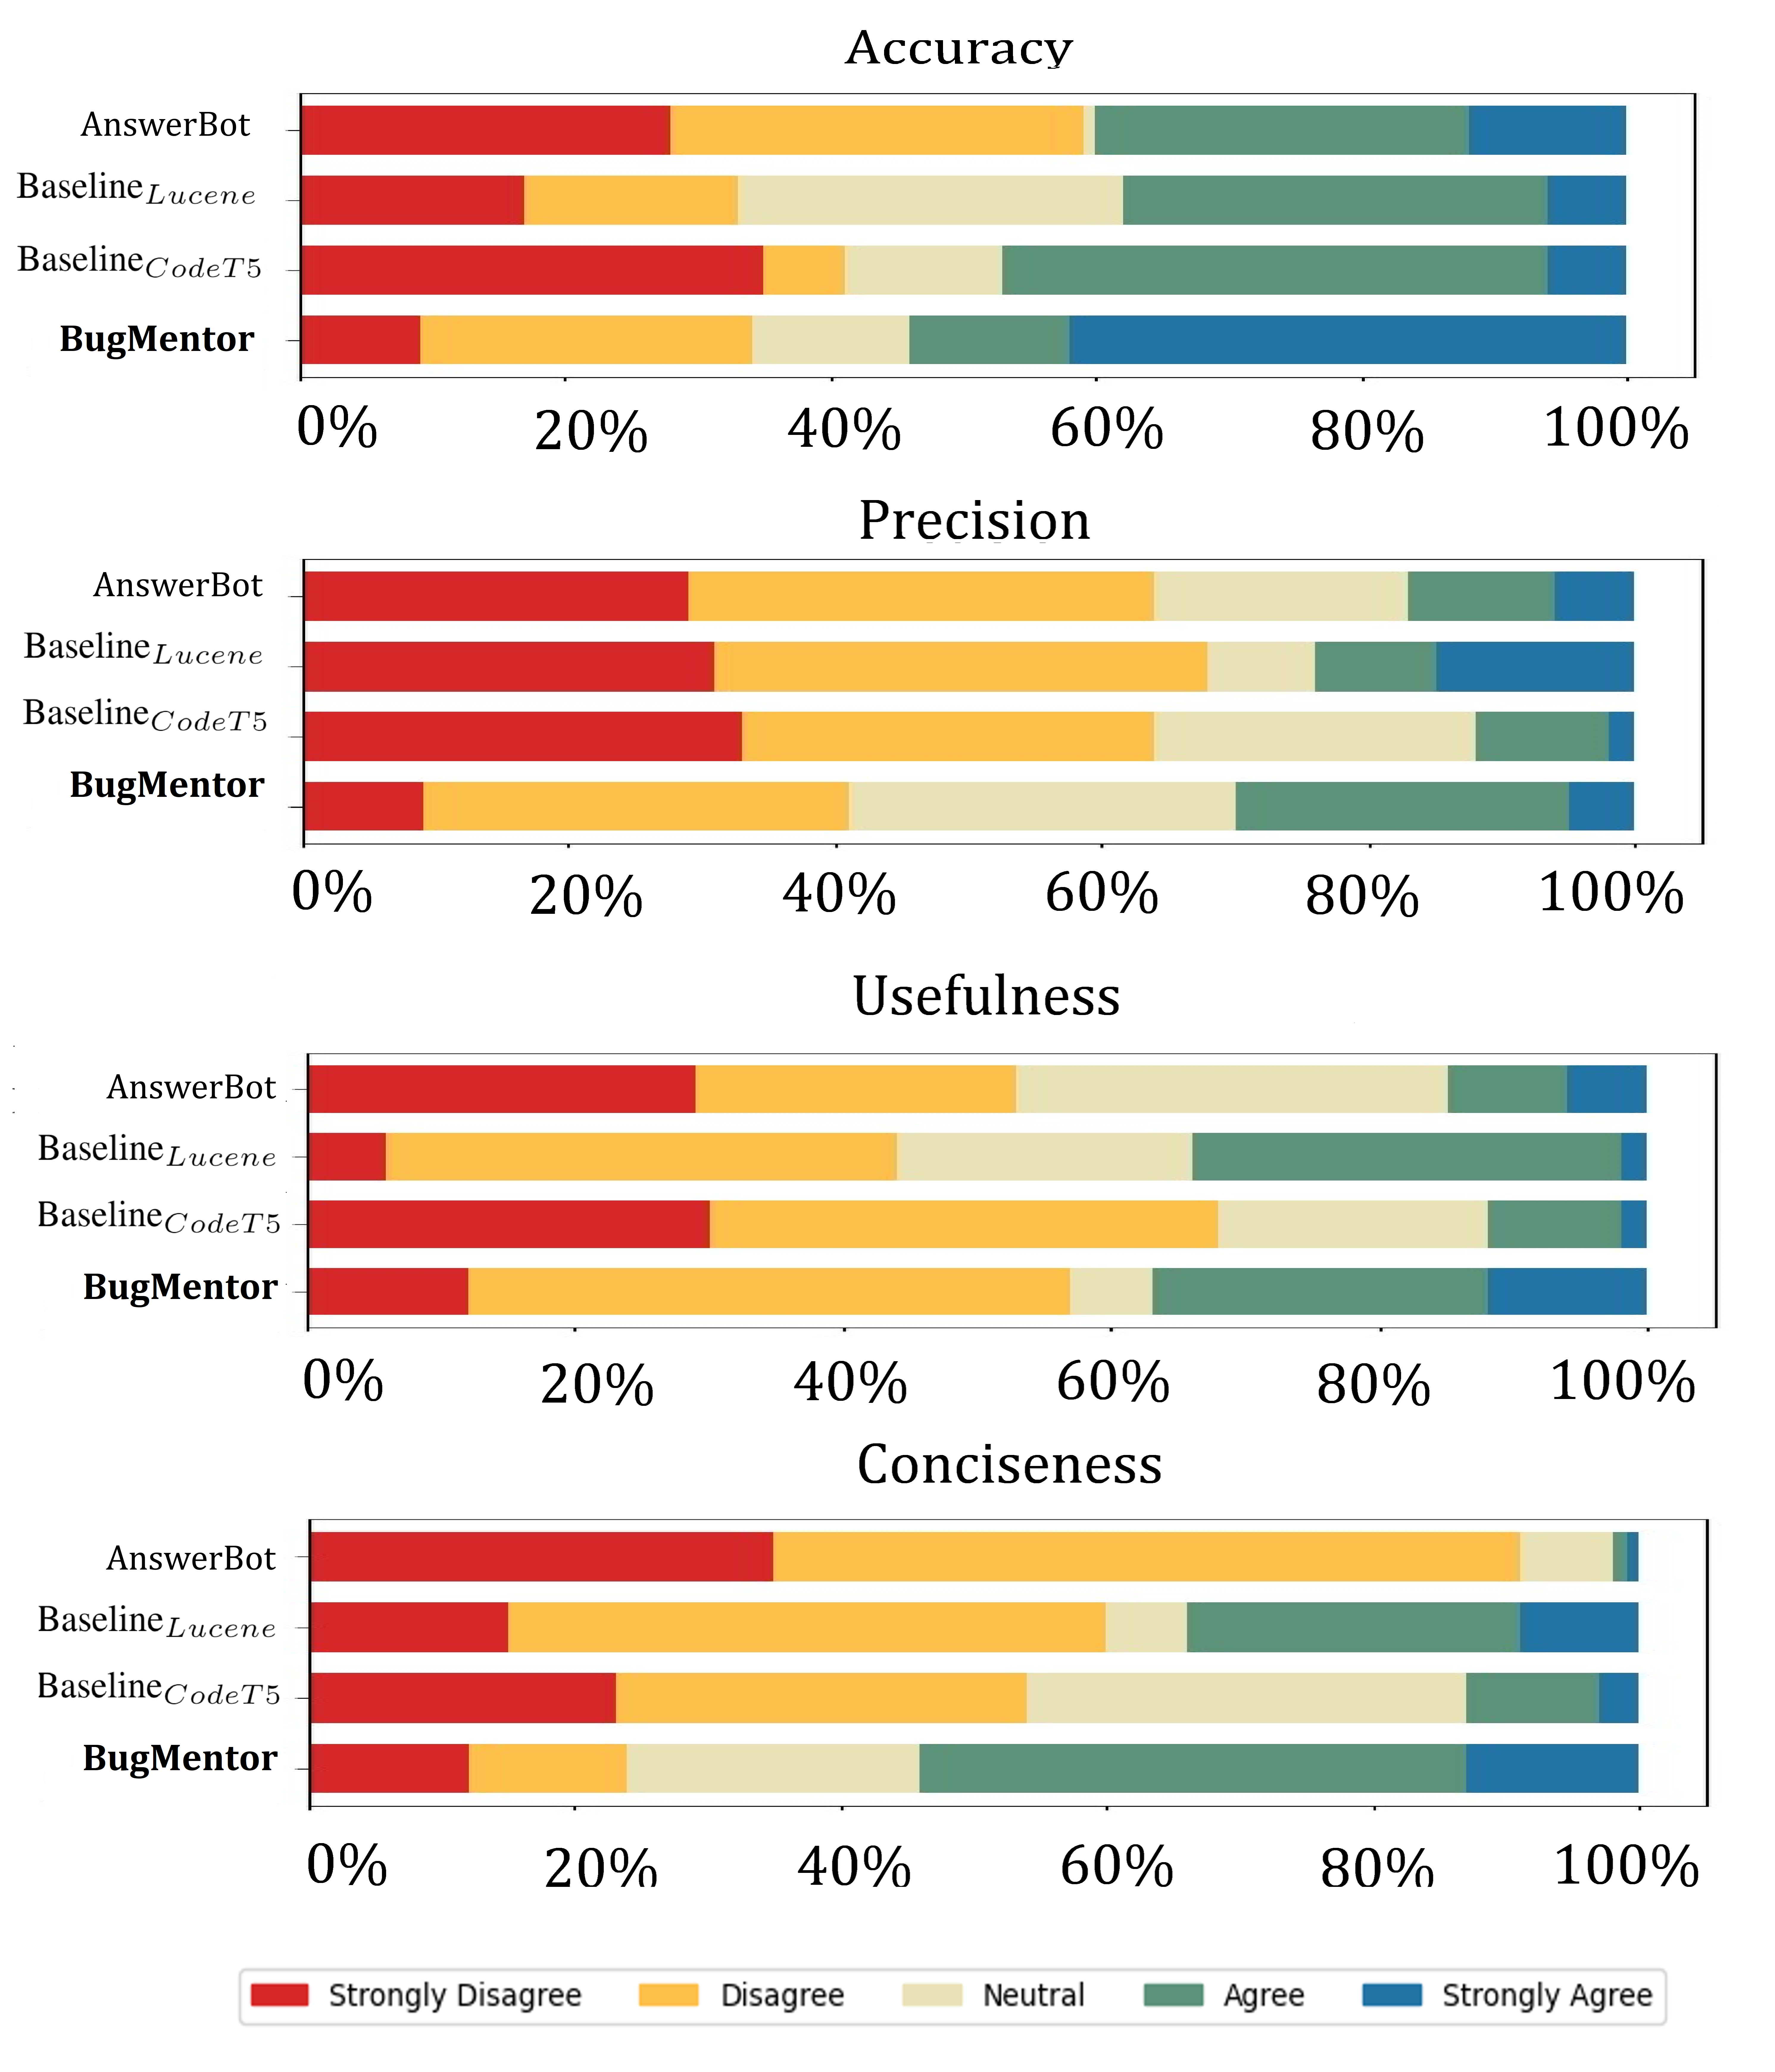
\includegraphics[width=\textwidth,keepaspectratio]{images/user_study_graph.png}
	\caption{Comparison of BugMentor with the baseline techniques using the Likert scores}
	\label{fig:dev}
\end{figure*}

\begin{table}[!ht]
\centering
\caption{Comparison of BugMentor with the Baseline Techniques using a Developer Study}
\label{tab:devstudy}
\renewcommand{\arraystretch}{1.2}
\resizebox{0.6\textwidth}{!}{
\begin{tabular}{|c|l|c|c|}
\hline
\textbf{Quality} & \multicolumn{1}{c|}{\textbf{Model}} & \textbf{Mean} & \textbf{Median} \\ \hline
\multirow{4}{*}{Accurate} & Baseline$_{Lucene}$ & 3.03 & 3 \\ \cline{2-4} 
 & Baseline$_{CodeT5}$ & 2.55 & 3 \\ \cline{2-4} 
 & AnswerBot & 2.65 & 2 \\ \cline{2-4} 
 & \textbf{BugMentor} & \textbf{3.10} & \textbf{3} \\ \hline
\multirow{4}{*}{Precise} & Baseline$_{Lucene}$ & 2.25 & 2 \\ \cline{2-4} 
 & CodeT5 & 2.56 & 3 \\ \cline{2-4} 
 & AnswerBot & 2.34 & 2 \\ \cline{2-4} 
 & \textbf{BugMentor} & \textbf{2.96} & \textbf{3} \\ \hline
\multirow{4}{*}{Useful} & Baseline$_{Lucene}$ & 2.62 & 2 \\ \cline{2-4} 
 & Baseline$_{CodeT5}$ & 2.46 & 2 \\ \cline{2-4} 
 & AnswerBot & 2.4 & 2 \\ \cline{2-4} 
 & \textbf{BugMentor} & \textbf{2.94} & \textbf{3} \\ \hline
\multirow{4}{*}{Concise} & Baseline$_{Lucene}$ & 2.68 & 2 \\ \cline{2-4} 
 & AnswerBot & 1.7 & 2 \\ \cline{2-4} 
 & Baseline$_{CodeT5}$ & 2.95 & 3 \\ \cline{2-4} 
 & \textbf{BugMentor} & \textbf{3.32} & \textbf{4} \\ \hline
\end{tabular}%
}
\end{table}

\textbf{Study Results and Discussion:} 
Table~\ref{tab:devstudy} summarizes our
findings from the developer study. We note that, on average, the participants found the answers from BugMentor to be the most accurate, precise, useful, and concise. Based on the median and mode values, we see that the participants 
agree with our answers the most.
%agree the most with answers from BugMentor. 
Similar to the findings in RQ$\mathbf{_2}$, the participants found the closest competitor of BugMentor to be Baseline$_{Lucene}$ in terms of precision, usefulness and conciseness and Baseline$_{CodeT5}$ in terms of accuracy. According to the median values, the developers agree with AnswerBot, Baseline$_{Lucene}$ and Baseline$_{CodeT5}$ in several cases. However, based on the mode values, we note that the participants disagree with their answers in many more cases.

\looseness=-1
Fig.~\ref{fig:dev} shows the distribution of participants’ agreement levels with different quality aspects of the answers. We see that the participants strongly agree with BugMentor for a substantial part of the time (e.g., $\sim$40\% for accuracy), and strongly disagree only a few times (e.g., $<$20\% times), which none of the baselines achieved. On the other hand, nearly half of the time, the participants disagree with AnswerBot, Baseline$_{Lucene}$ and Baseline$_{CodeT5}$ regarding various quality aspects of their provided answers.\par

\looseness=-1
We also perform Mann-Whitney Wilcoxon test~\cite{cuzick1985wilcoxon} to check if the developers' preferences to Baseline$_{Lucene}$, Baseline$_{CodeT5}$ and AnswerBot are significantly lower than that of BugMentor using BonFerroni Correction~\cite{weisstein2004bonferroni}. We find that the preference levels for BugMentor are significantly higher than all three baselines, i.e., p $=$ 0.0010$<$0.016 for Baseline$_{Lucene}$, p $=$ 0.0016$<$0.016 for  Baseline$_{CodeT5}$, and p $=$ 0.00016$<$0.016 for AnswerBot.

\renewcommand{\arraystretch}{1.2}
\begin{table}[htbp]
\caption{Manual Analysis}
\label{tab:manualanalysis}
\centering
\begin{threeparttable}
\begin{tabular}{|c|c|c|c|c|} \hline
\textbf{Dataset}   & \textbf{AC}    & \textbf{AP}    & \textbf{AP + AddInfo} & \textbf{AddInfo} \\ \hline \hline
Java & 7  & 9  & 12  & 20  \\ \hline
Python & 8  & 9 & 17  & 14  \\ \hline
C++  & 4 & 4 & 16  & 24 \\ \hline
JavaScript & 8  & 5  & 16  & 19  \\ \hline
\textbf{Average\%} & \textbf{14.06} & \textbf{14.06} & \textbf{31.77}        & \textbf{40.10}   \\ \hline
\end{tabular}   
\begin{tablenotes}
  \small
  \item \begin{center}
     \textbf{AC} $=$ Answers Completely, \textbf{AP} $=$ Answers Partially,\\ \textbf{AddInfo} $=$ Additional Information 
  \end{center}
\end{tablenotes}
\end{threeparttable}
\end{table}


\textbf{Manual Analysis:}
\looseness=-1
To further investigate the usefulness of BugMentor's answers, we perform a manual analysis on 192 bug reports (i.e. 48 samples for each programming language). We select these samples from the whole collection with a 95\% confidence level and 4.95\% error margin. We collect the bug reports, follow-up questions, ground truth and generated answers. Table~\ref{tab:manualanalysis} shows the summary of our analysis. \par

\looseness=-1
We analyze our generated answers to the follow-up questions, contrast them against the ground truth, and determine whether they respond to the question completely, partially or simply provide additional information. We find that BugMentor, on average, was able to answer the questions completely for 14.06\% of the cases from each programming language. It was able to answer 14.06\% of the questions partially while adding complementary information to 31.77\% of the answers. Furthermore, in 40\% cases, our technique delivered such answers that did not match with the ground truth answers but were complementary or somewhat relevant to the questions. For example, let us consider the bug report shown below discussing the issue of links in Atom. It does not provide the version of the operating system that the reporter uses. The ground truth answer indicates the OS version and the issue persistence in the safe mode of the browser. We see that BugMentor's answer captures the context and points out that the problem might lie with Ubuntu version rather than other running applications. Thus, BugMentor can provide complementary information that can benefit the developer.


\begin{frshaded}
\noindent
\textbf{Title:} Links do not work in Atom \\
\textbf{Description:} After upgrading to Atom, links no longer open in a new tab in Chrome. For example, clicking on any of the release notes links does nothing. \\
\textbf{Question:} What OS do you experience this issue in safe mode? \\
\textbf{Actual Answer:} Ubuntu; safe mode exhibits the same issue. \\
\textbf{Generated Answer:} Since upgrading to Ubuntu, I've had no issues. However, similar problems with other apps make me suspect it's related to the Ubuntu version. Even in safe mode, Atom still exhibits the problem.
\end{frshaded}

\FrameSep.3em
\begin{frshaded}
	\noindent
        \looseness=-1
	\textbf{Summary of RQ$\mathbf{_4}$:} Developers with professional experience found the answers of BugMentor to be accurate, precise, concise, and useful, with respect to the ground truth answers. Their preference levels for BugMentor were also higher than those of the three baseline techniques by a statistically significant margin.  
\end{frshaded}


\section{Related Work} \label{Chap1:RelatedWork}

\looseness=-1
Question Answering (QA) has been an active research topic in both Information Retrieval (IR) and Natural Language Processing (NLP) communities~\cite{ravichandran2002learning, brill2002analysis,waltz1978english, iyyer2014neural,asaduzzaman2013answering, tian2017apibot, lu2021beat, bansal2021neural, xu2017answerbot, abdellatif2020msrbot}. There also have been several works that focus on question-answering in the context of software engineering. Breu et al.~\cite{breu2010information} first analyzed follow-up questions from bug reports and found that 32.34\% of them were never responded to. Recently, Imran et al.~\cite{imran2021automatically} proposed Bug-AutoQ that recommends follow-up questions against a deficient bug report leveraging development history using information retrieval. However, their technique does not answer the follow-up questions.\par


\looseness=-1
Murgia et al.~\cite{murgia2016among} leverage the search feature of StackOverflow Q\&A site to suggest relevant questions against error messages from a version control system. However, their technique was trained to provide only simple, recurring questions related to Git error messages. Tian et al.~\cite{tian2017apibot} propose APIBot that can answer questions related to an API by analyzing the relevant API documentation. However, their solution was limited to API-related questions only. Bansal et al.~\cite{bansal2021neural} design a context-aware QA system to answer basic questions about subroutines. Lu et al.~\cite{lu2021beat} propose another QA approach that can provide answers by executing structured queries generated from a bug report template. Xu et al.~\cite{xu2017answerbot} designed AnswerBot to synthesize answers for technical, non-factoid questions from StackOverflow. 
However, they only use the title of a question overlooking the detailed problem context (e.g., question body), and thus their answers might be unaware of the problem context. We compare BugMentor with AnswerBot using experiments, and the detailed comparison can be found in Section~\ref{results:rq2}. Abdellatif et al. ~\cite{abdellatif2020msrbot} designed MSRBot to answer the most common questions related to software development and maintenance. However, their answers might be limited by the available information in the mined repositories. Song et al.~\cite{song2022toward} designed BURT to support bug reporters of Android applications, but their approach might not generalize to other software applications.

Recently, Language Model-based approaches (LLMs) such as ChatGPT have emerged as a powerful text generation tool. After conducting a limited qualitative analysis (Section~\ref{results:rq2}), we note that while ChatGPT exhibit an understanding of a given bug report, they often struggle to come up with precise answers to follow-up questions. BugMentor has a better understanding of past bug reports and thus captures a broader context. In the future, we plan on conducting a thorough comparison between BugMentor and contemporary LLM-based approaches like ChatGPT.


In short, existing relevant works focus on improving deficient bug reports and answering specific questions related to API, subroutines and Git error messages. 
To the best of our knowledge, our proposed technique is the first to automatically answer the follow-up questions from bug reports, which makes our work \emph{novel}. We also combine structured information retrieval with neural text generation (e.g., CodeT5) to generate the answers, which were found to be meaningful, accurate, precise, useful, and concise according to two types of evaluation --- automated metrics and developer study. Our technique also outperforms three baselines.  


\section{Threats to Validity} \label{Chap1:Threats}
We identify a few threats to the validity of our findings. In this section, we examine these threats and discuss the steps that were taken to mitigate them.\par

\looseness=-1
\textbf{External Validity:}
Threats to external validity refer to the lack of generalizability in the findings~\cite{ferguson2004external}. One threat could stem from our selection of subject systems. We select 20 software systems written in four programming languages: Python, Java, JavaScript, and C++, which might not represent all systems at GitHub. However, the underlying algorithm of BugMentor is not bound to any programming language and thus can be easily adapted to any other platforms.\par
Another threat stems from the small sample size of the held-out dataset for evaluation (e.g., 550). However, to mitigate this concern, we selected them carefully through random sampling from all four subsets (95\% confidence level, 4.06\% error margin, Section~\ref{sec:groundtruth}). We also maintain diversity in selecting our 20 subject systems (Section~\ref{sec:groundtruth}). 

\looseness=-1
\textbf{Construct Validity:} Construct validity refers to the extent to which the experiment measures what it intends to measure~\cite{smith2005construct}. 
Inappropriate use of evaluation metrics could be a threat to construct validity. However, we chose our evaluation metrics --- BLEU, METEOR, Semantic Similarity, and WMD --- based on relevant literature~\cite{papineni2002bleu,banerjee2005meteor,haque2022semantic,huang2016supervised}. We also chose the four quality aspects of generated answers based on relevant literature~\cite{imran2021automatically,joshi2015likert}. Thus, threats to construct validity might be mitigated.

\looseness=-1
\textbf{Internal Validity:} Threats to internal validity relate to experimental errors and subjective biases~\cite{christ2007experimental}. We use manually annotated ground truth to answer both RQ1 and RQ2, which could be a source of threat. However, to mitigate this, the annotators were given appropriate training for their annotation tasks. We also employ majority voting~\cite{kuhrmann2017pragmatic} for decision-making and calculate Cohen's $\kappa$ to demonstrate the agreement levels between annotators~\cite{kuhrmann2017pragmatic}.
In the developer study, the assessment of answers can be influenced by subjective bias. However, we anonymize the source of all answers to avoid any bias towards any technique.
\looseness=-1
Another source of threat could be the replication of the baseline techniques. For the replication of CodeT5, we collected the pre-trained model from HuggingFace~\cite{huggingface_t5}, and for the replication of Lucene, we used ElasticSearch~\cite{ElasticSearch}, a standard library. To replicate AnswerBot~\cite{xu2017answerbot}, we used the replication package from the original authors~\cite{maxxbw54}. Furthermore, we followed the documentation closely for any customizations. Thus, threats to internal validity might be mitigated.
 
\section{Summary} \label{Chap1:Summary}

To summarize, in this study, we propose BugMentor, a novel technique to answer follow-up questions from deficient bug reports by combining structured information retrieval and neural text generation. Our technique leverages the relevance between past and current bug reports to gather additional context, which helps us generate an appropriate answer to the question. Our evaluation using four performance metrics shows that BugMentor can generate understandable and good answers to follow-up questions, as per Google's Standard. Our technique outperforms three existing baselines. We also evaluate BugMentor using a user study using 10 developers. The developers found the answers from BugMentor to be more accurate, precise, concise and useful compared to the baseline answers. Thus, BugMentor has the potential to support bug resolution with complementary information in the form of answers to follow-up questions. However, newcomers or novice developers often struggle to understand bug reports due to their lack of in-depth knowledge about an application. Thus we perform another study to further improve the quality of bug reports by providing explanations to their domain-specific terms or jargon.
